\chapter{Intact polar lipid response factors and mass spectral interpretation of novel structures}\label{app1}

\clearpage

\doublespace

\paragraph*{Analytical response factors.} Table \ref{tab:RF} provides information about response factors for the suite of intact polar lipid (IPL) standards used in this work. Response factors were interpreted as the linear slopes of high-performance liquid chromatography-mass spectrometry (HPLC-MS) integrated peak area as a function of injected mass with a y-intercept of zero. The squared correlation coefficient, $R^{2}$, is reported for each regression. Two sets of response factors are given: one for a sample batch run in 2013 and another in 2014. Samples MS1, MS3, MS4, and MS5 use the response factors for 2014, while all other samples use those for 2013.

\paragraph*{Mass spectral interpretation of novel structures.} Mass spectra and putative chemical structures of lipids identified in this work are shown in Figures \ref{fig:MeNG-G-P-AR} through \ref{fig:G-GA-DAG}. All lipid structures shown in this appendix are tentatively assigned based on MS/MS fragmentation patterns. Carbon positions of alkyl chain modifications, bonding, and configuration between glycolipid headgroup moieties, \textit{etc.}, are guesses. Dotted arrows refer to inferred fragmentation of the displayed structure and point in the direction of the fragment with the monoisotopic mass, in Da, listed at the end of the arrow. pNLC stands for `precursor neutral loss chromatogram'. This a chromatogram based on the difference between the mass of a lipid precursor ion before and after the loss of a diagnostic fragment. Usually, in the case of IPLs, this is the headgroup or a piece of the headgroup. M+H and M-H refer to the monoisotopic mass of the displayed structure plus or minus a hydrogen atom, respectively, and assumes the resulting fragment has an overall charge of +1.

\clearpage

\afterpage{
\singlespace
\begin{table}
\centering
\begin{threeparttable}
  \caption{HPLC-MS IPL standards and response factors}
 
% Table generated by Excel2LaTeX from sheet 'RF info (2)'
\begin{tabular}{rllrrrr}
\toprule
      &       &       & \multicolumn{2}{c}{Batch 1\tnote{b}} & \multicolumn{2}{c}{Batch 2\tnote{c}} \\
\cmidrule(l{2pt}r{2pt}){4-5} \cmidrule(l{2pt}r{2pt}){6-7}No.\tnote{a} & Standard & Chains & RF    & \textit{R\textsuperscript{2}} & RF    & \textit{R\textsuperscript{2}} \\
\midrule
1     & 1Gly-DAG & mix of C34:6, C36:6 & 6.37$\times 10$\textsuperscript{5} & 0.95  & 9.45$\times 10$\textsuperscript{5} & 0.99 \\
2     & 1Gly-GDGT-PG & mix of 0-3 rings, & 6.72$\times 10$\textsuperscript{4} & 0.96  & 1.16$\times 10$\textsuperscript{4} & 0.91 \\
      &       & $\sim$20\% H-shaped &       &       &       &  \\
3     & PC-DAG & C42:0 & 7.31$\times 10$\textsuperscript{5} & 0.99  & 2.71$\times 10$\textsuperscript{5} & 0.91 \\
4     & 2Gly-DAG & mix of C34:2, C34:3 & 1.33$\times 10$\textsuperscript{5} & 0.99  & 9.90$\times 10$\textsuperscript{4} & 0.99 \\
      &       & C34:6, C36:6 &       &       &       &  \\
5     & SQ-DAG & mix of C34:2,  & 1.31$\times 10$\textsuperscript{5} & 0.95  & 1.90$\times 10$\textsuperscript{5} & 0.99 \\
      &       & C34:3, C36:6 &       &       &       &  \\
6     & PI-DAG & C32:0 & 7.94$\times 10$\textsuperscript{3} & 0.88  & 5.95$\times 10$\textsuperscript{3} & 0.99 \\
7     & DPG   & C72:4 & 3.97$\times 10$\textsuperscript{5} & 0.95  & 7.24$\times 10$\textsuperscript{4} & 0.99 \\
8     & PDME-DAG & C32:0 & 1.11$\times 10$\textsuperscript{6} & 0.97  & 1.96$\times 10$\textsuperscript{6} & 0.99 \\
9     & PE-DAG & C32:0 & 4.06$\times 10$\textsuperscript{5} & 0.99  & 2.92$\times 10$\textsuperscript{5} & 0.95 \\
10    & PG-DAG & C32:0 & 1.49$\times 10$\textsuperscript{5} & 0.98  & 1.02$\times 10$\textsuperscript{5} & 0.99 \\
11    & PME-DAG & C32:0 & 5.45$\times 10$\textsuperscript{5} & 0.94  & 5.93$\times 10$\textsuperscript{5} & 0.99 \\
12    & PS    & C32:0 & 2.03$\times 10$\textsuperscript{4} & 0.98  & 2.30$\times 10$\textsuperscript{4} & 0.97 \\
13    & DGTS-d9 & C32:0 & 1.65$\times 10$\textsuperscript{6} & 0.89  & 7.16$\times 10$\textsuperscript{6} & 0.96 \\
\bottomrule
\end{tabular}%



\begin{tablenotes}
\small
\item [a] Corresponds to numbered standards in Table \ref{tab:IPL} of main text.
\item [b] Batch 1 was analyzed in 2013 and includes all Bison Pool, Empress Pool, and Octopus Spring samples, as well as Mound Spring sample MS2. Linear response factors and \textit{R\textsuperscript{2}} were taken from two replicate calibrations of 0.1, 0.5, 1, 5, 10, and 50 ng standard injections.
\item [c] Batch 2 was analyzed in 2014 and includes Mound Spring samples MS1, MS3, MS4, and MS5. Linear response factors and \textit{R\textsuperscript{2}} were taken from a single calibration of 0.1, 0.5, 1, 5, and 10 ng standard injections.

\end{tablenotes}

  \label{tab:RF}
  \end{threeparttable}
\end{table}

% replace \cmidrule{4-7} with:
% \cmidrule(l{2pt}r{2pt}){4-5} \cmidrule(l{2pt}r{2pt}){6-7}
\doublespace
\clearpage
}


\afterpage{
\singlespace
\begin{figure}[h]
\centering
    \begin{subfigure}[b]{1\linewidth}
       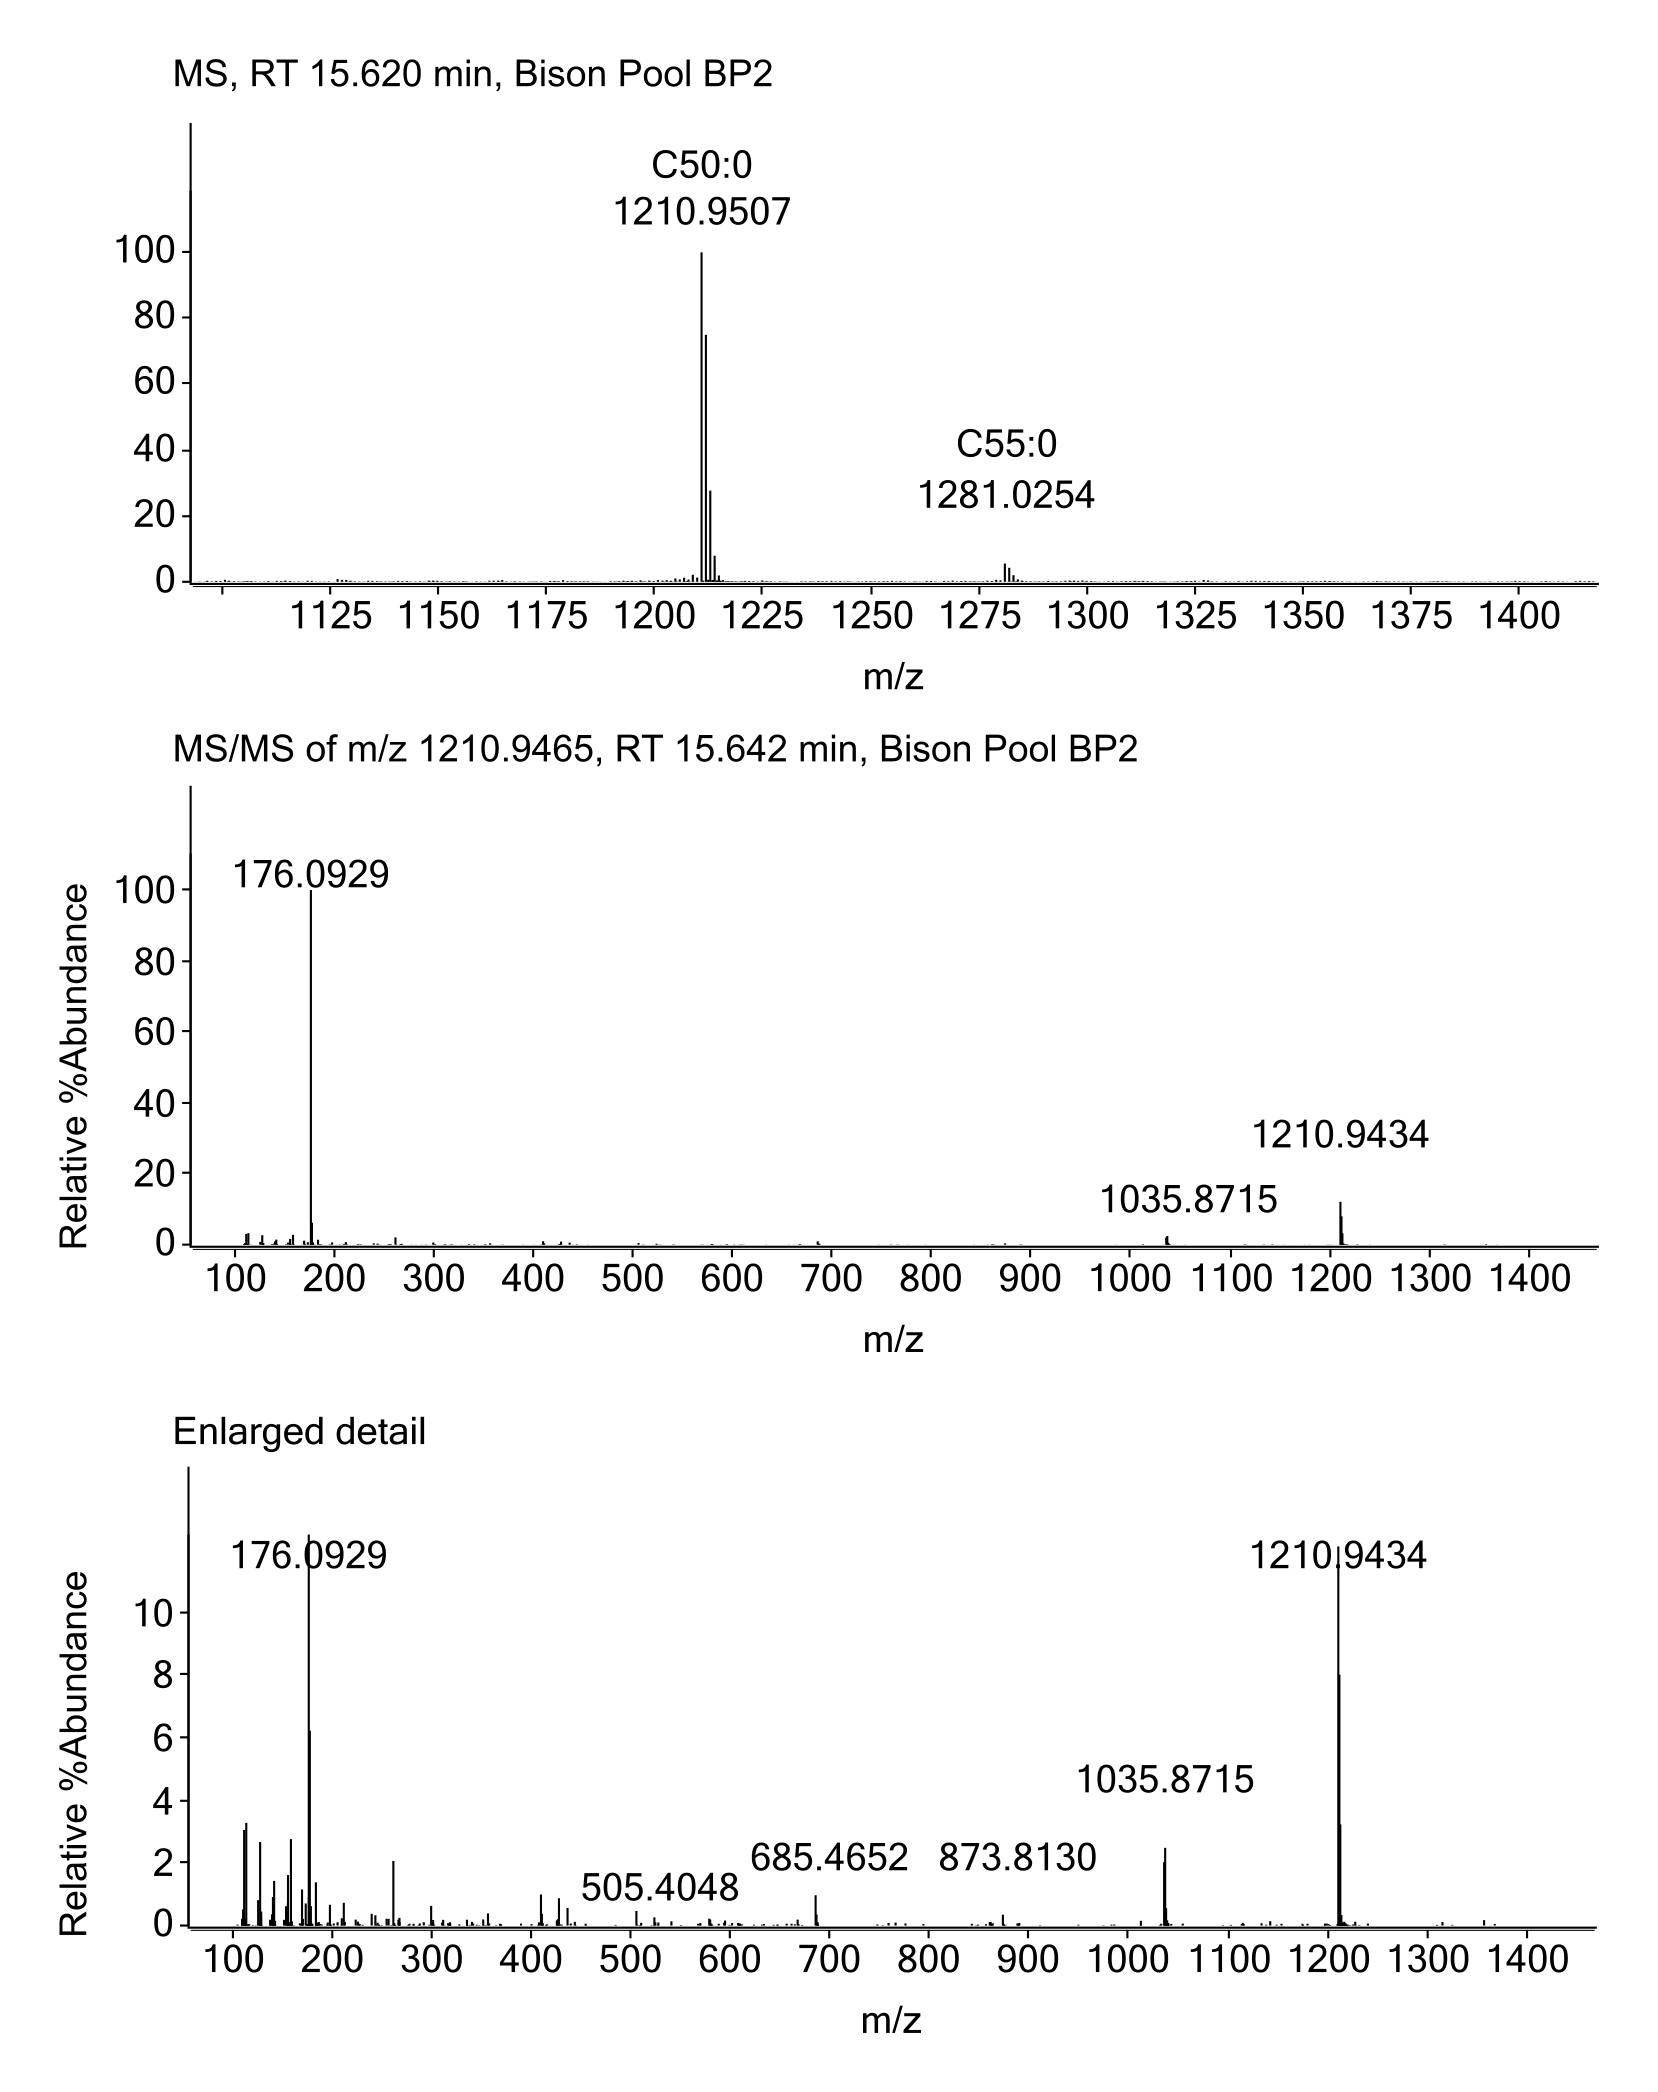
\includegraphics[width=\linewidth]{figs_app1/MeNG-G-P-AR_1}
       \caption{mass spectra}
        \label{fig:gull}
    \end{subfigure}
\end{figure}
\newpage
\begin{figure}[h] \ContinuedFloat
    \begin{subfigure}[b]{1\linewidth}
       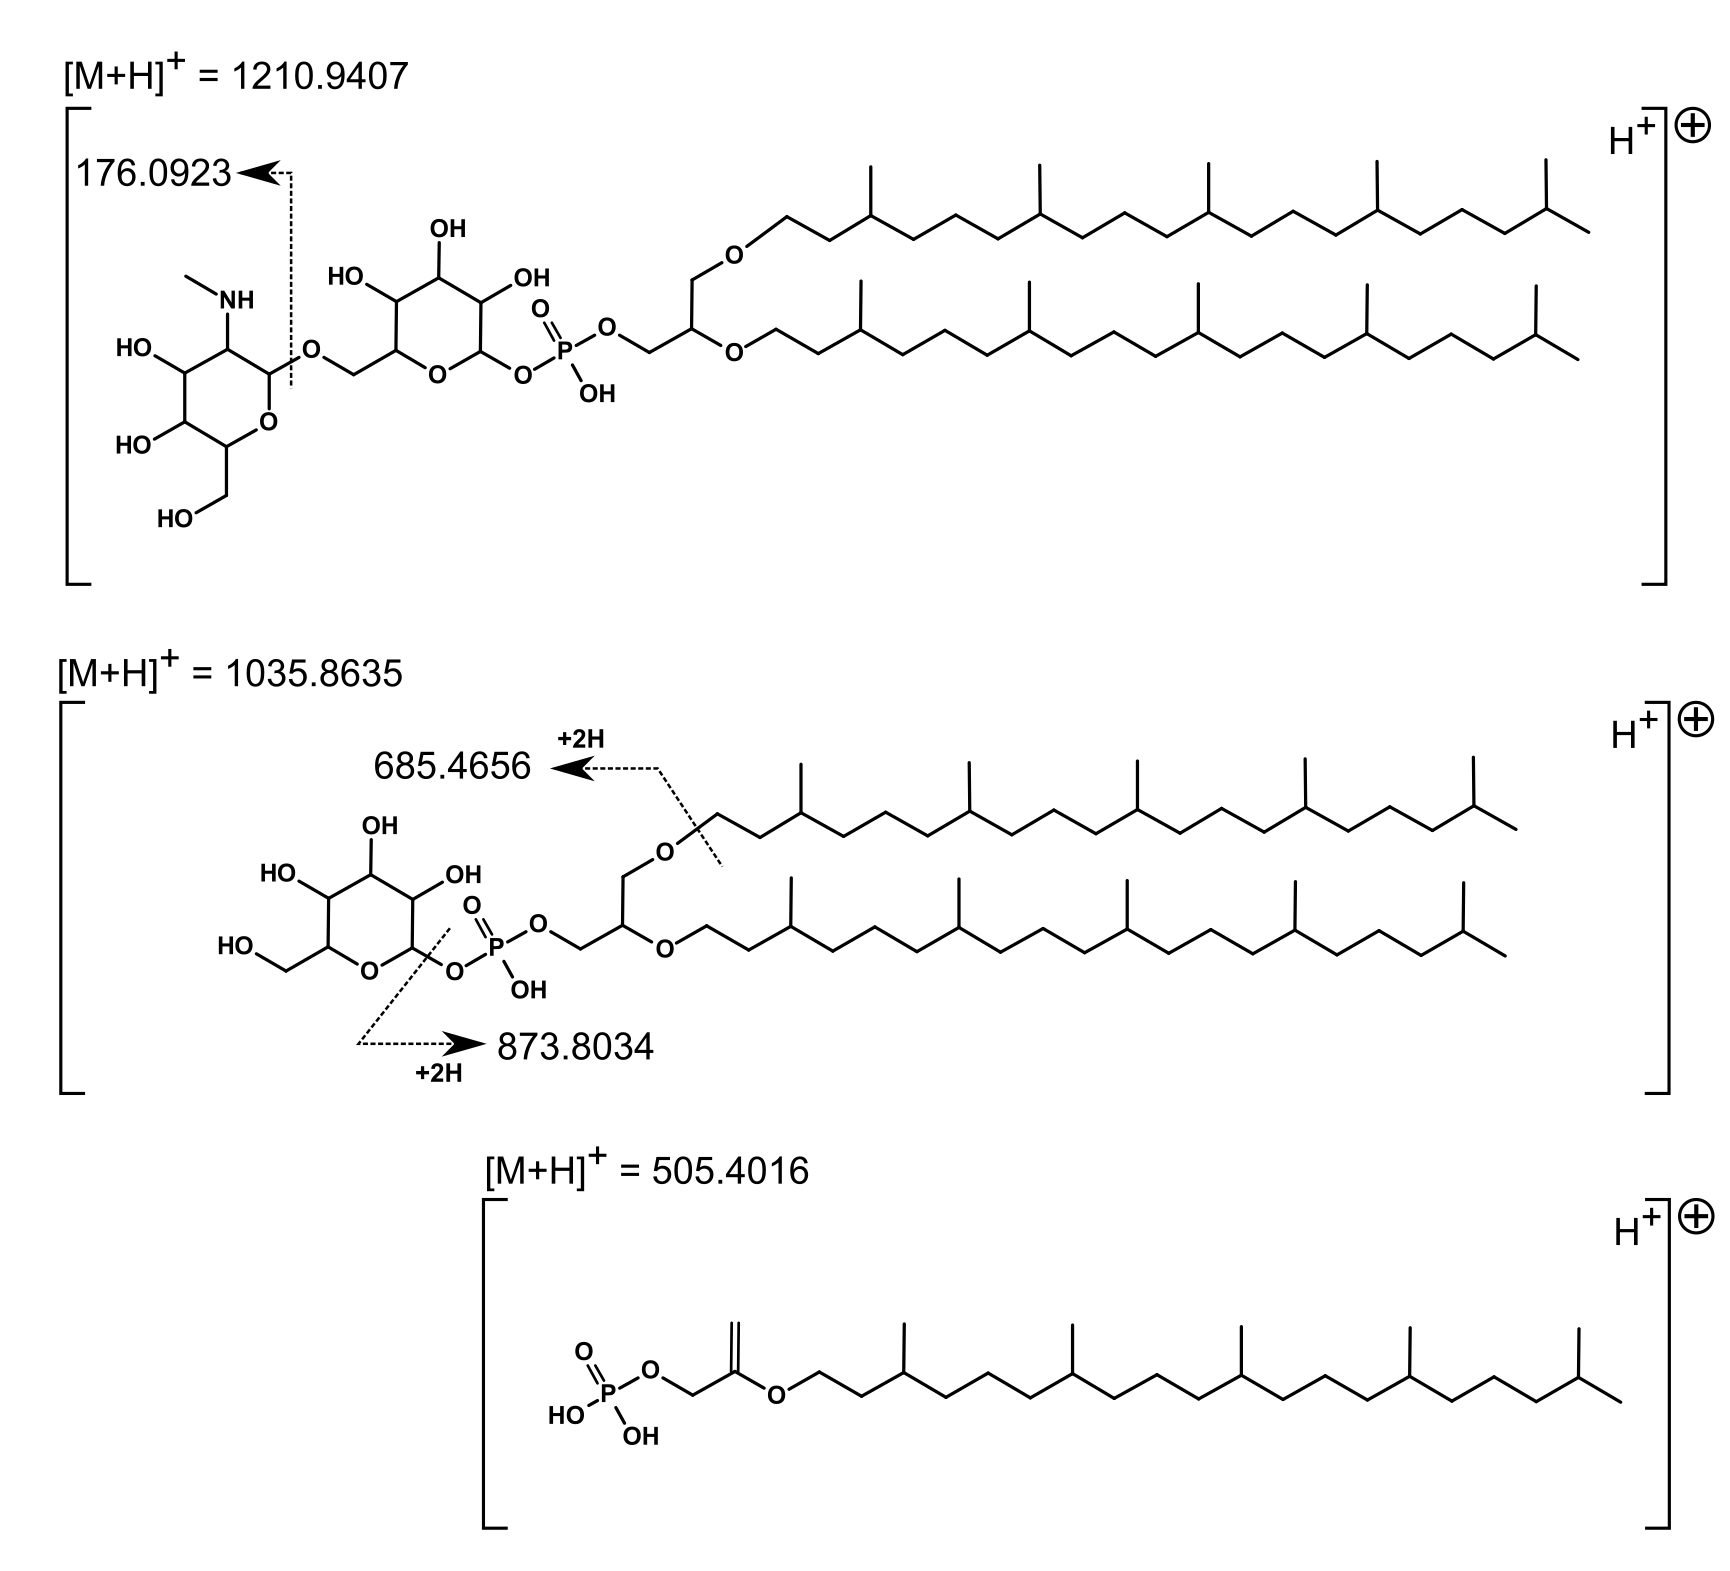
\includegraphics[width=\linewidth]{figs_app1/MeNG-G-P-AR_2}
       \caption{putative fragments}
        \label{fig:gull}
    \end{subfigure}
\caption{Mass spectra and putative structure for (N-methyl)glycosaminyl monoglycosyl phosphatidylarchaeol (MeNG-G-P-AR).}
\label{fig:MeNG-G-P-AR}
\end{figure}
\doublespace
\clearpage
}

\afterpage{
\singlespace
\begin{figure}[h]
\centering
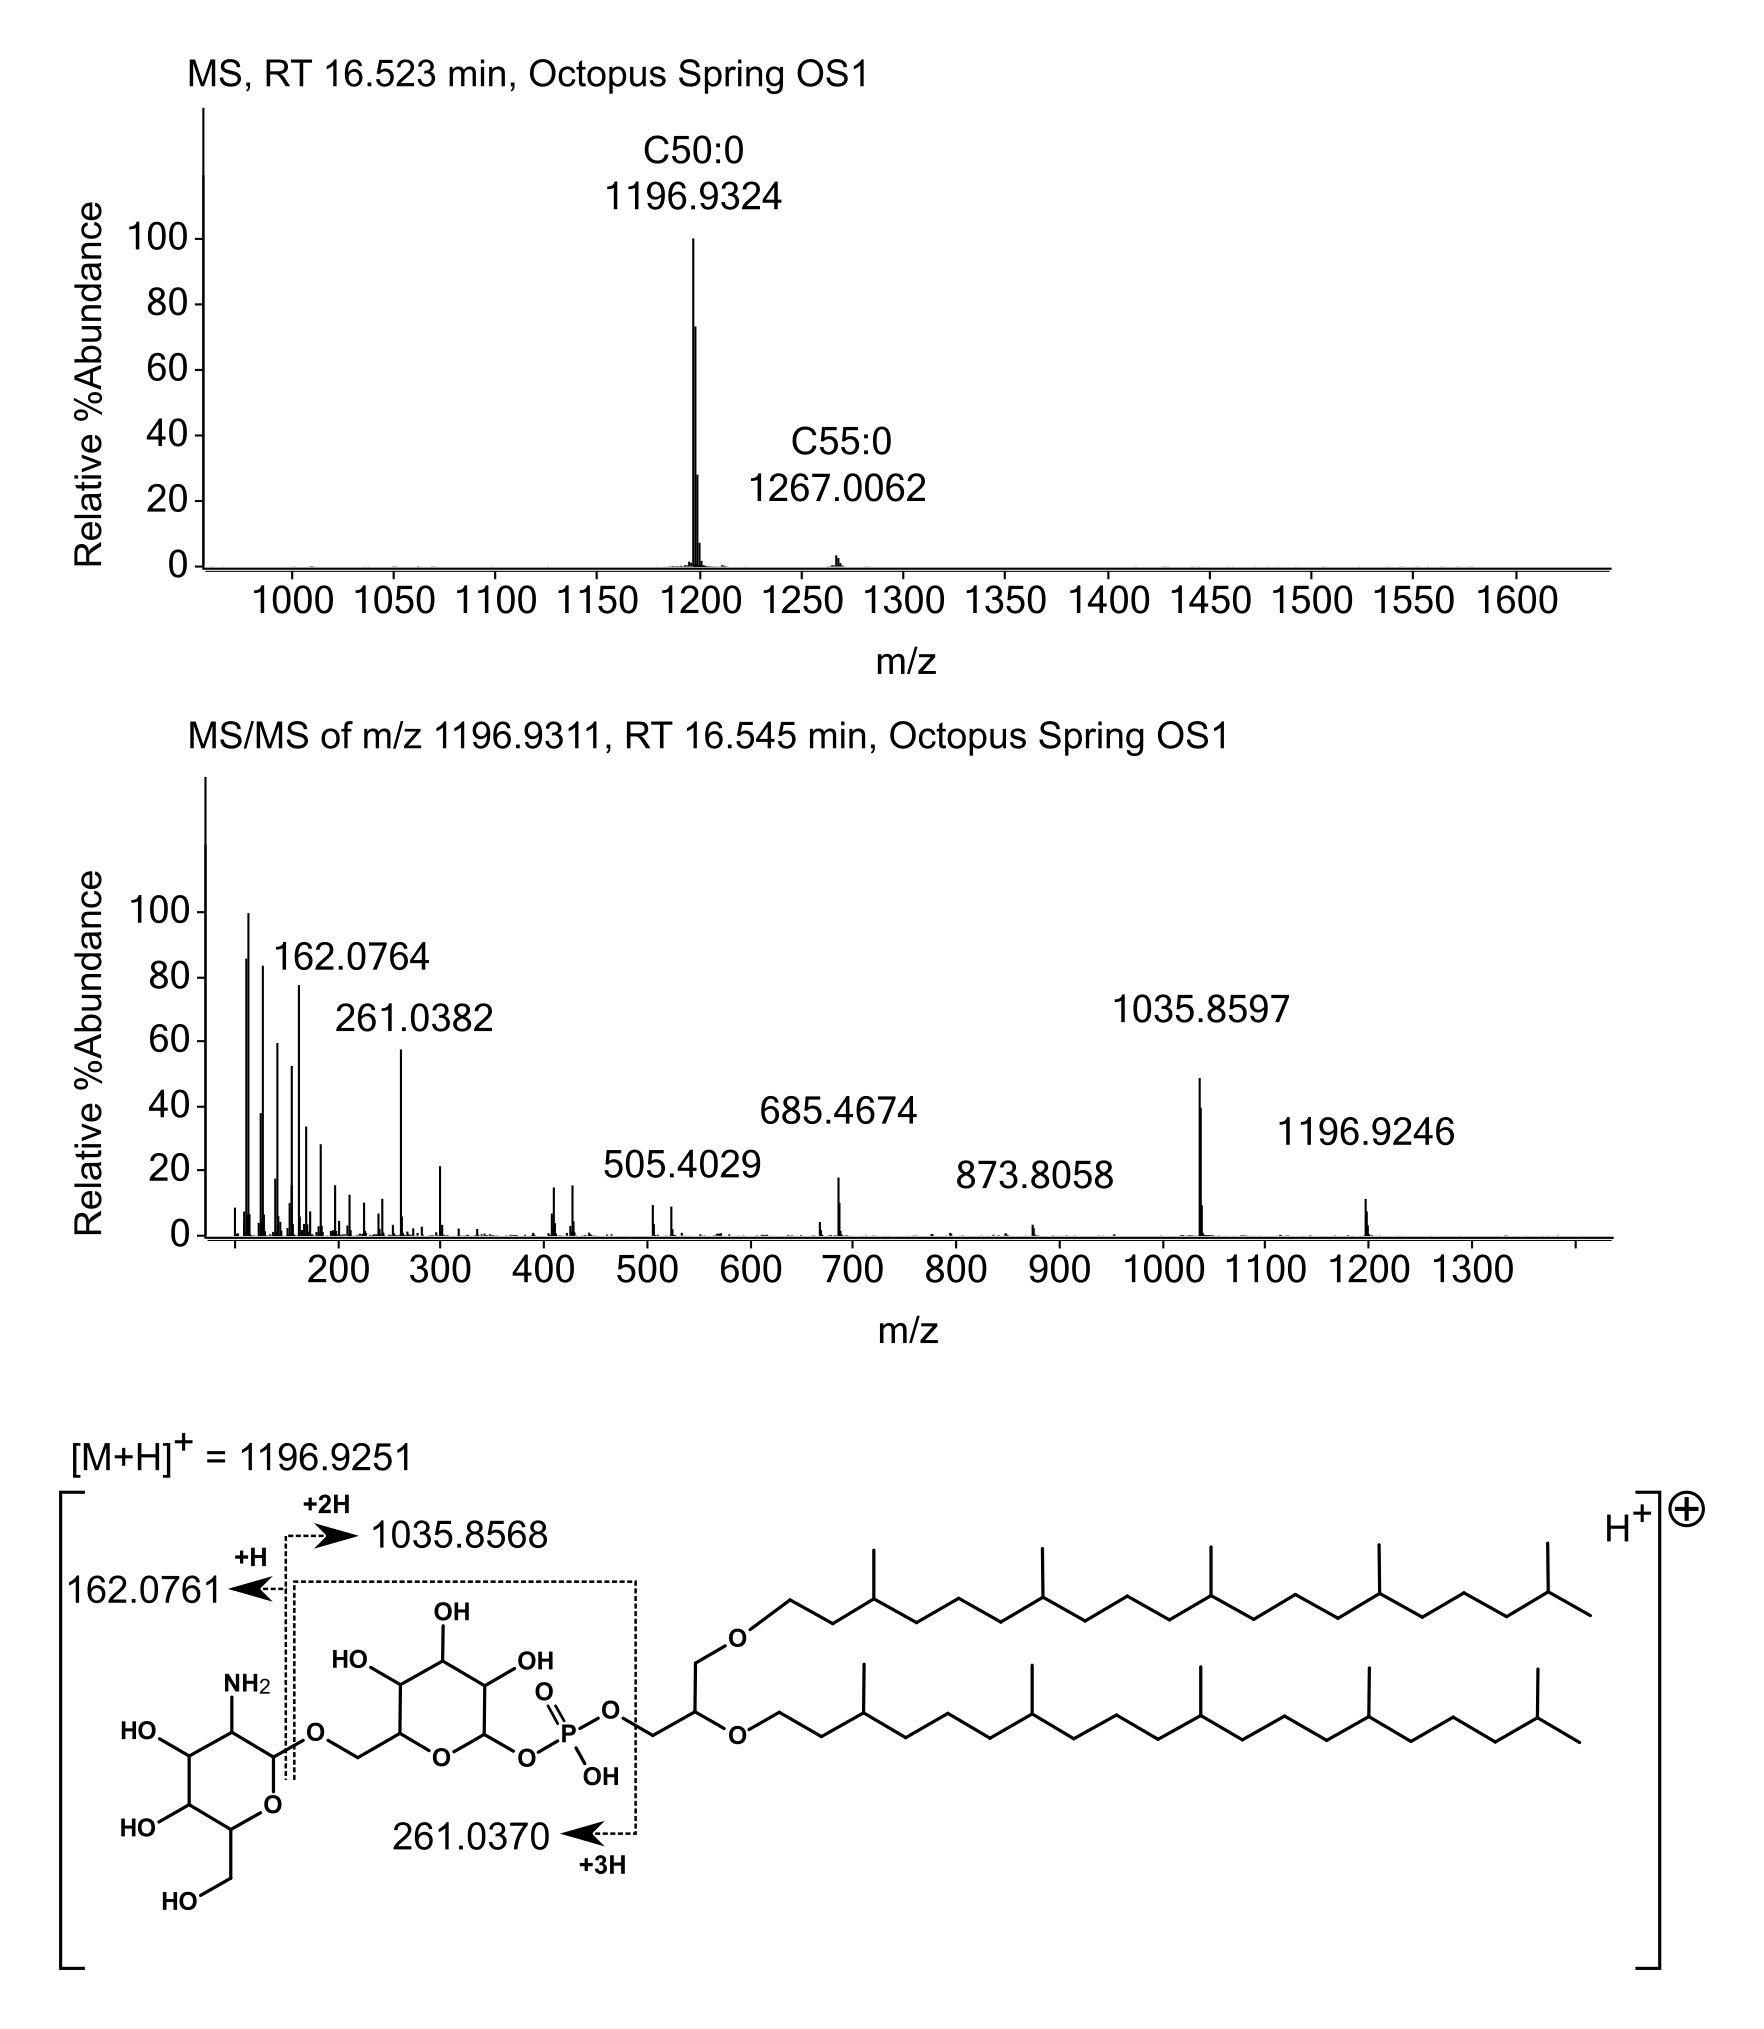
\includegraphics[width=\linewidth]{figs_app1/NG-G-P-AR}
\caption[Mass spectra and putative structure for (N)glycosaminyl monoglycosyl phosphatidylarchaeol (NG-G-P-AR)]{Mass spectra and putative structure for (N)glycosaminyl monoglycosyl phosphatidylarchaeol (NG-G-P-AR). This and MeNG-G-P-AR share many fragments in MS/MS due to their structural similarity (see Figure \ref{fig:MeNG-G-P-AR}).}
\label{fig:NG-G-P-AR_percent}
\end{figure}
\doublespace
\clearpage
}

\afterpage{
\singlespace
\begin{figure}[h]
\centering
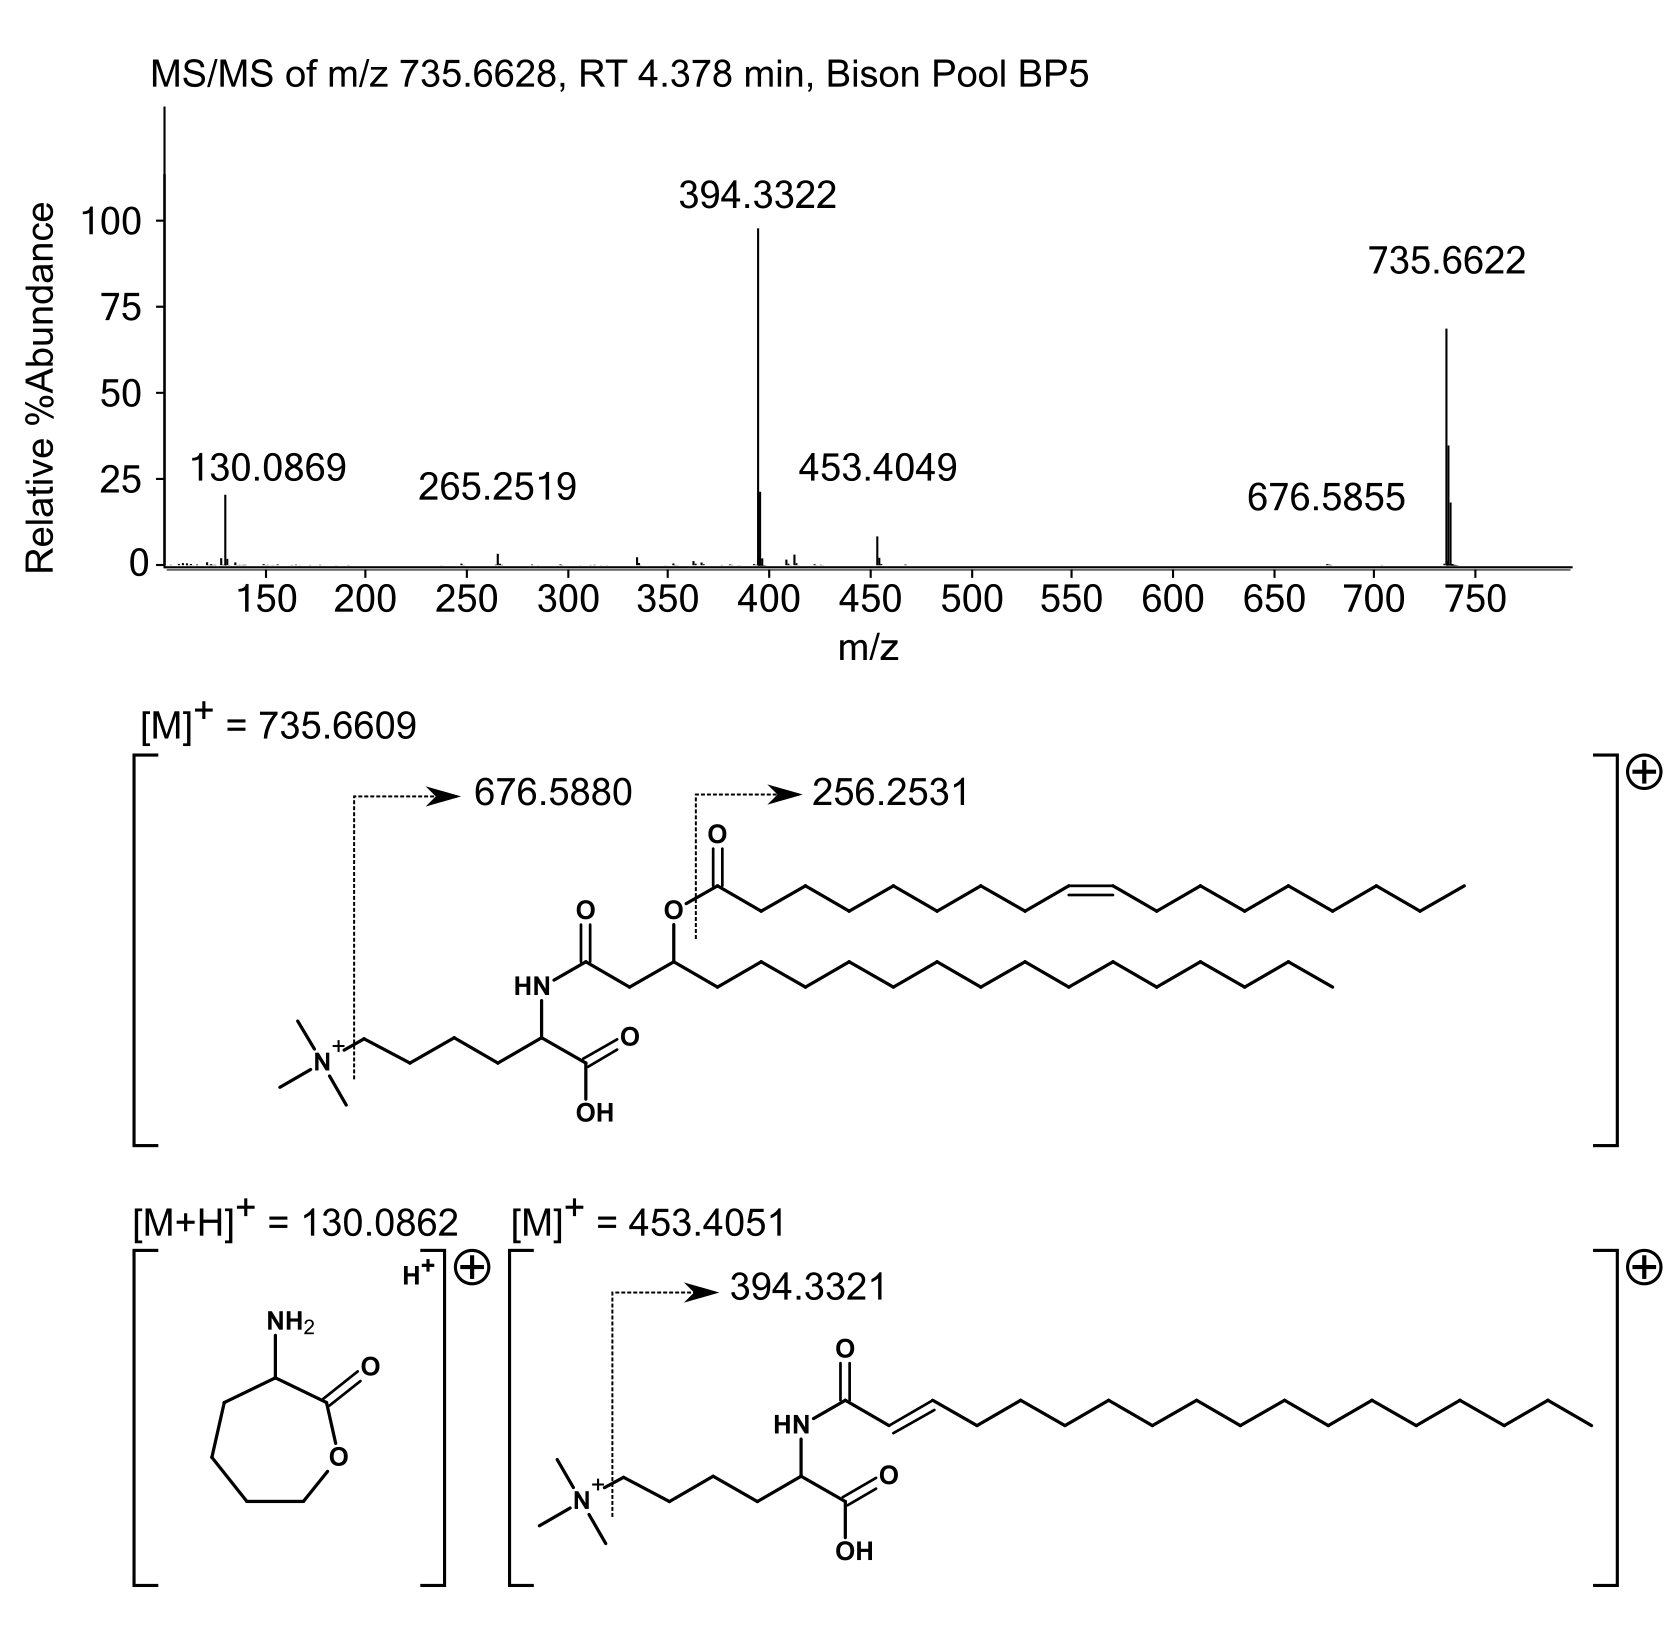
\includegraphics[width=\linewidth]{figs_app1/TM-KL}
\caption{Mass spectrum and putative structure for (6-N,6-N,6-N)trimethyllysine lipid (TM-KL).}
\label{fig:TM-KL}
\end{figure}
\doublespace
\clearpage
}


\afterpage{
\singlespace
\begin{figure}[h]
\centering
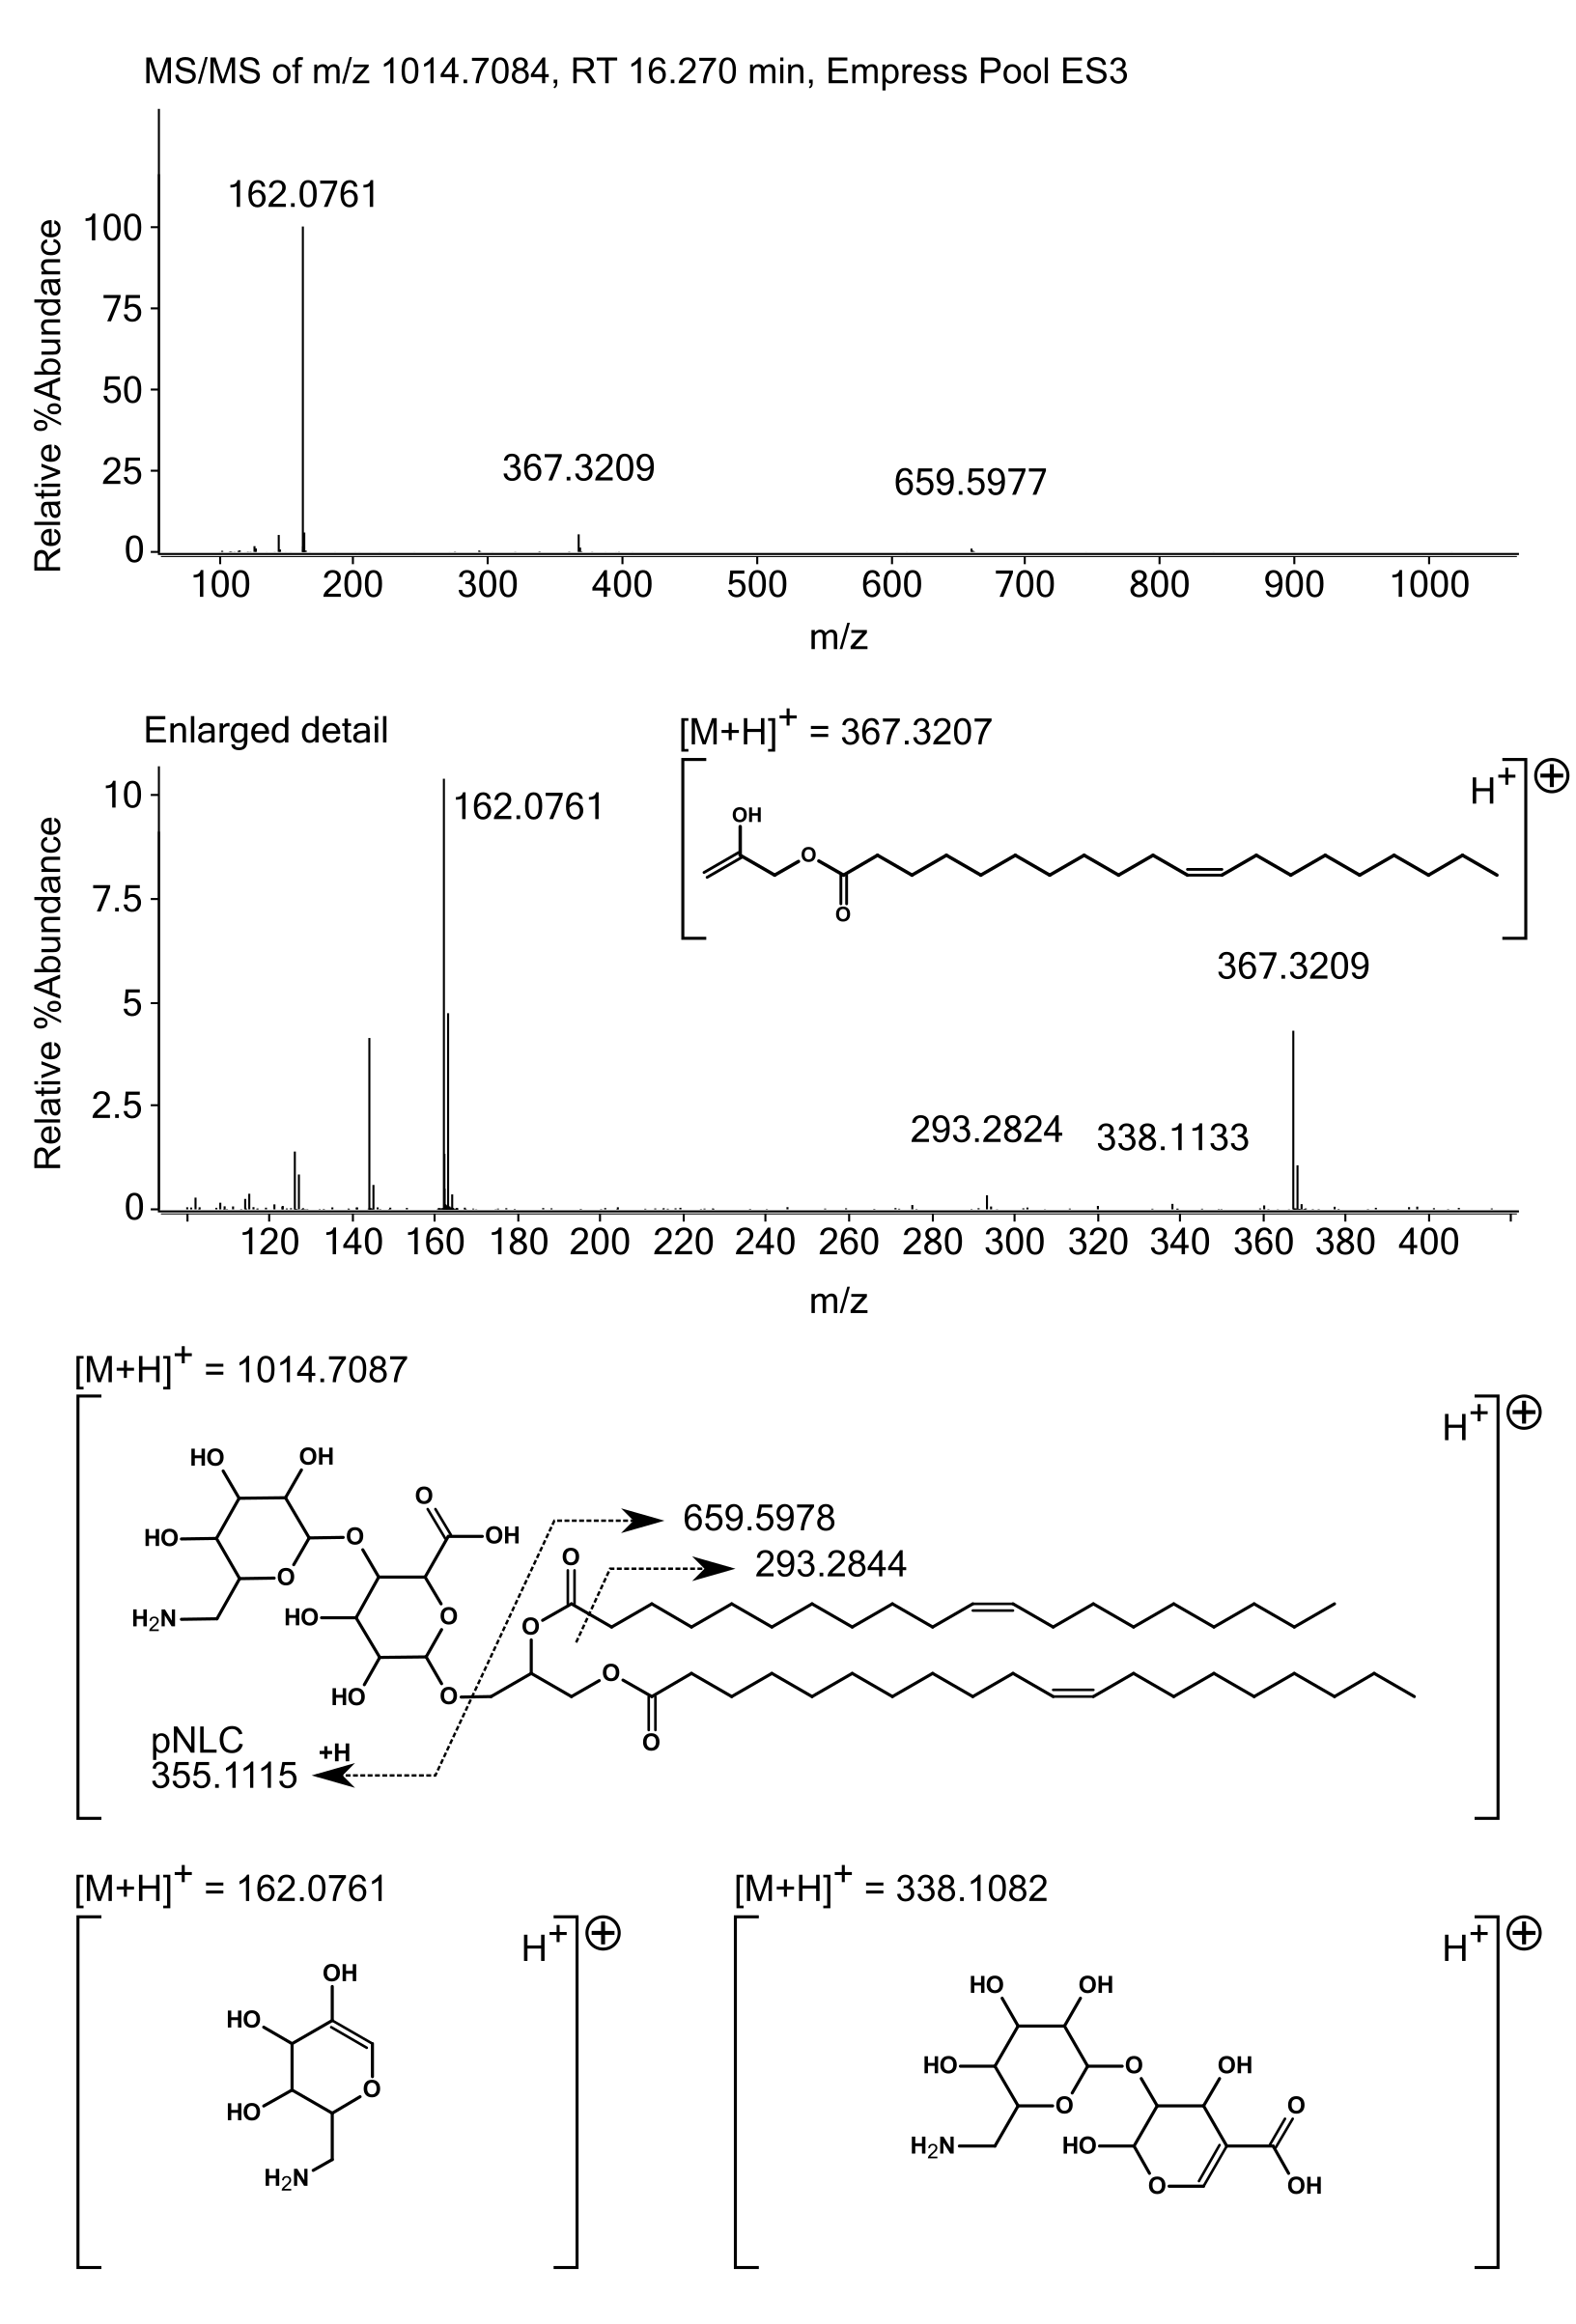
\includegraphics[width=0.9\linewidth]{figs_app1/NG-GA-DAG}
\caption{Mass spectra and putative structure for (6-N,6-N,6-N)trimethyllysine lipid (NG-GA-DAG).}
\label{fig:NG-GA-DAG}
\end{figure}
\doublespace
\clearpage
}


\afterpage{
\singlespace
\begin{figure}[h]
\centering
    \begin{subfigure}[b]{1\linewidth}
       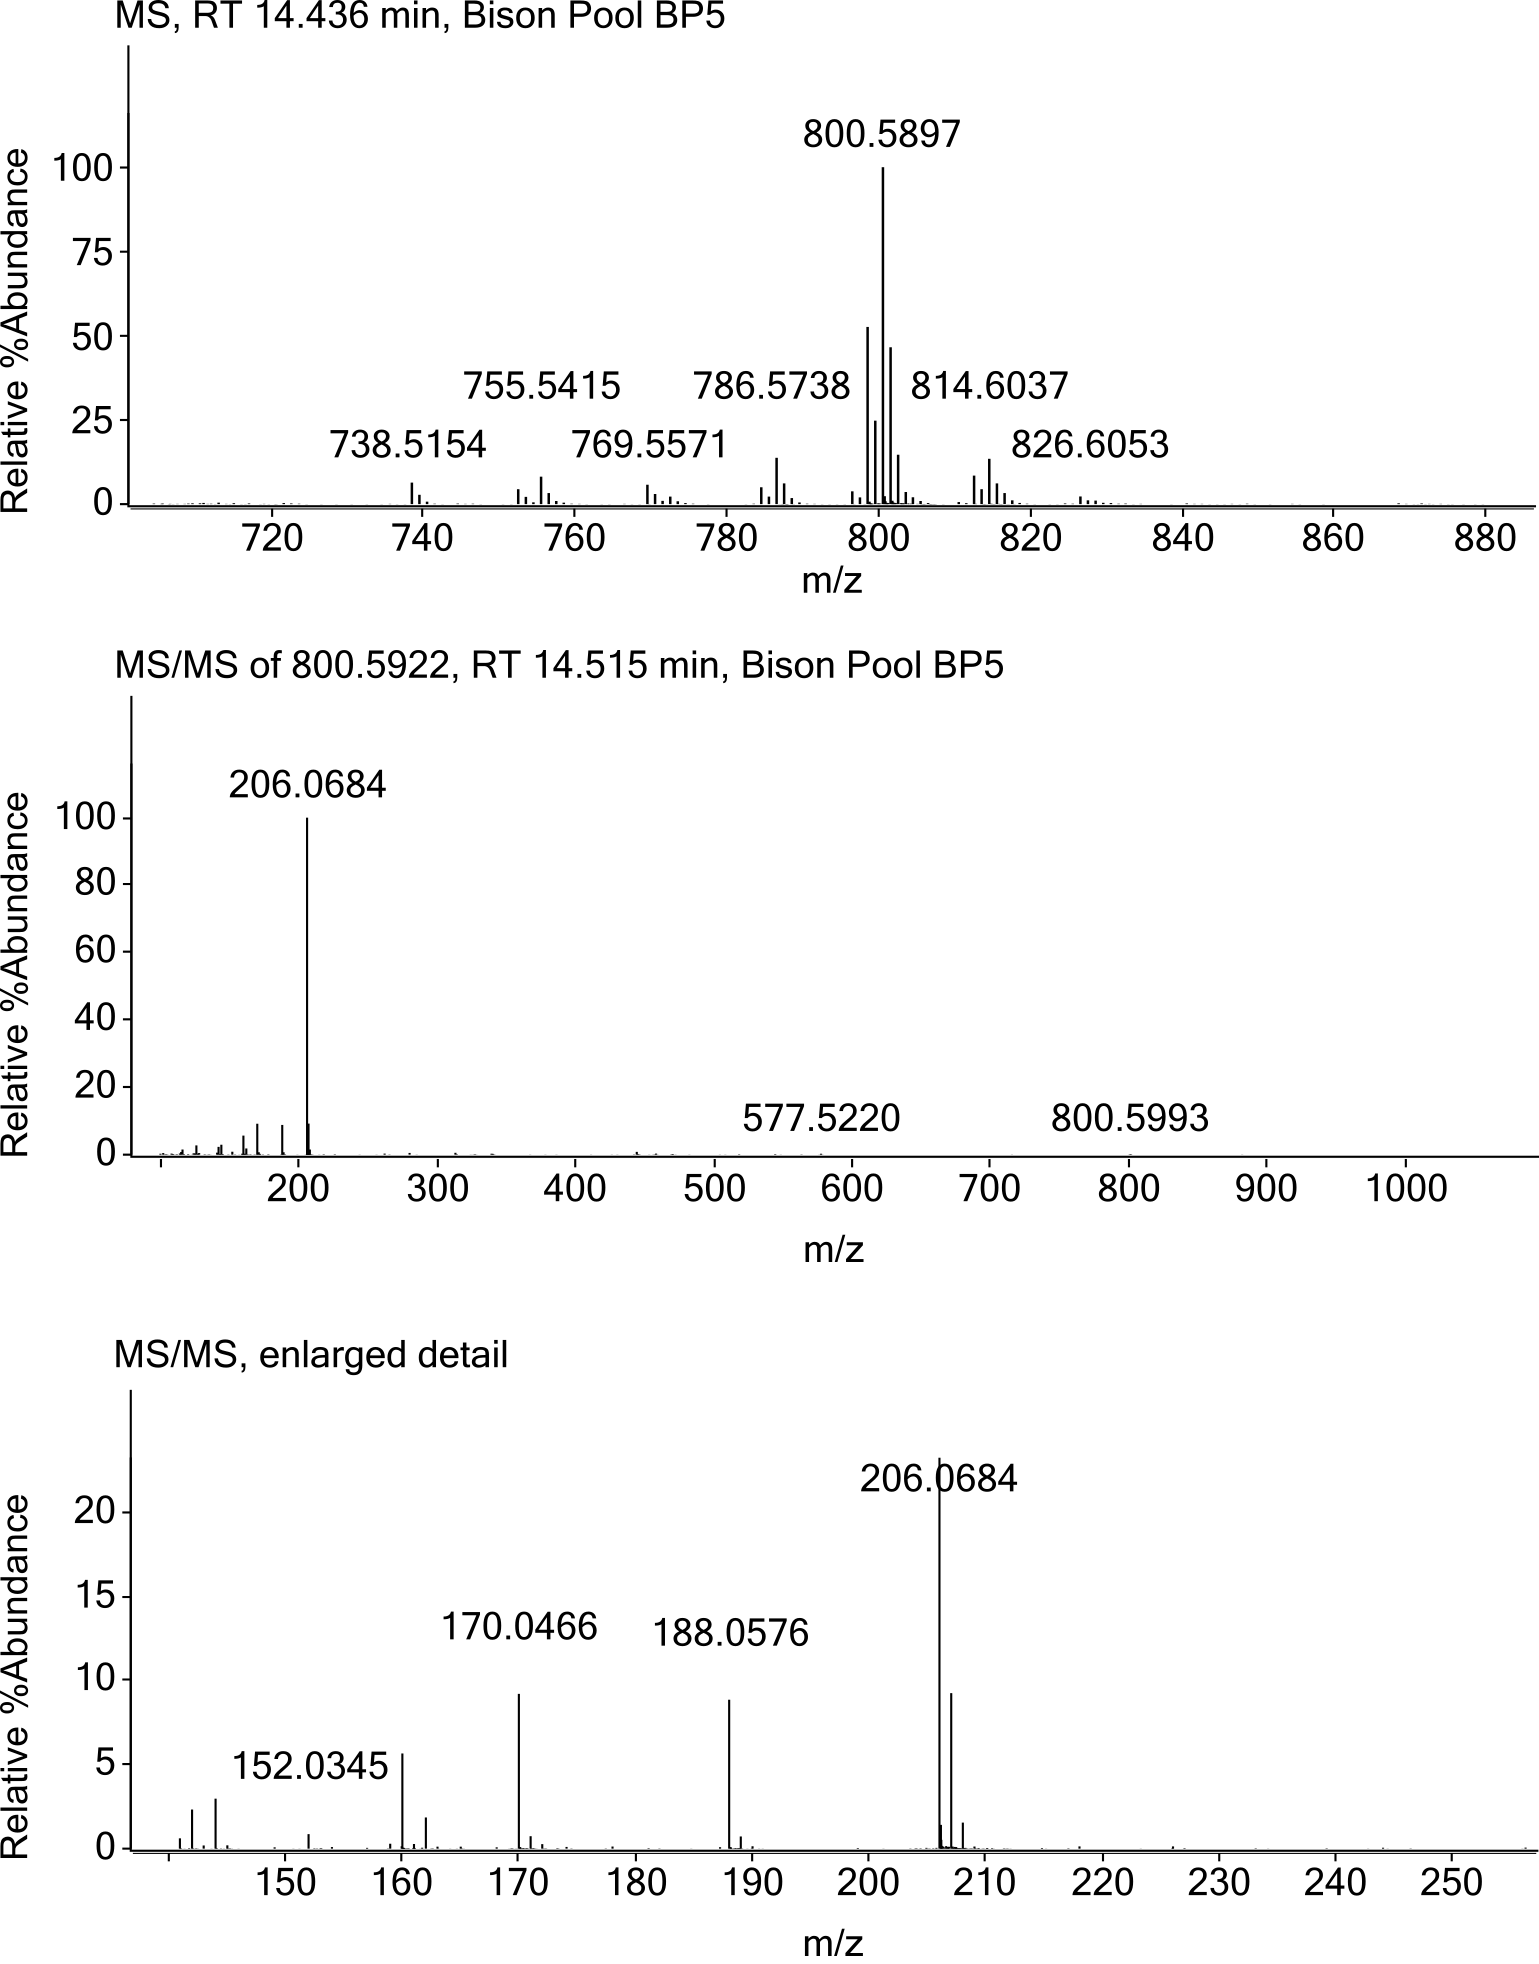
\includegraphics[width=\linewidth]{figs_app1/223-DAG_1}
       \caption{The MS/MS spectrum of C34:1 ‘223’-DAG within the m/z 250 – 800 range. Neutral loss of the headgroup results in [M + H]+ - m/z 223.07 = m/z 577.51, corresponding to the ion shown below, where nC in acyl chains R1 and R2 sum to 34 with one unsaturation.}
        \label{fig:223-DAG-MS}
    \end{subfigure}
\end{figure}
\newpage
\begin{figure}[h] \ContinuedFloat
    \begin{subfigure}[b]{1\linewidth}
       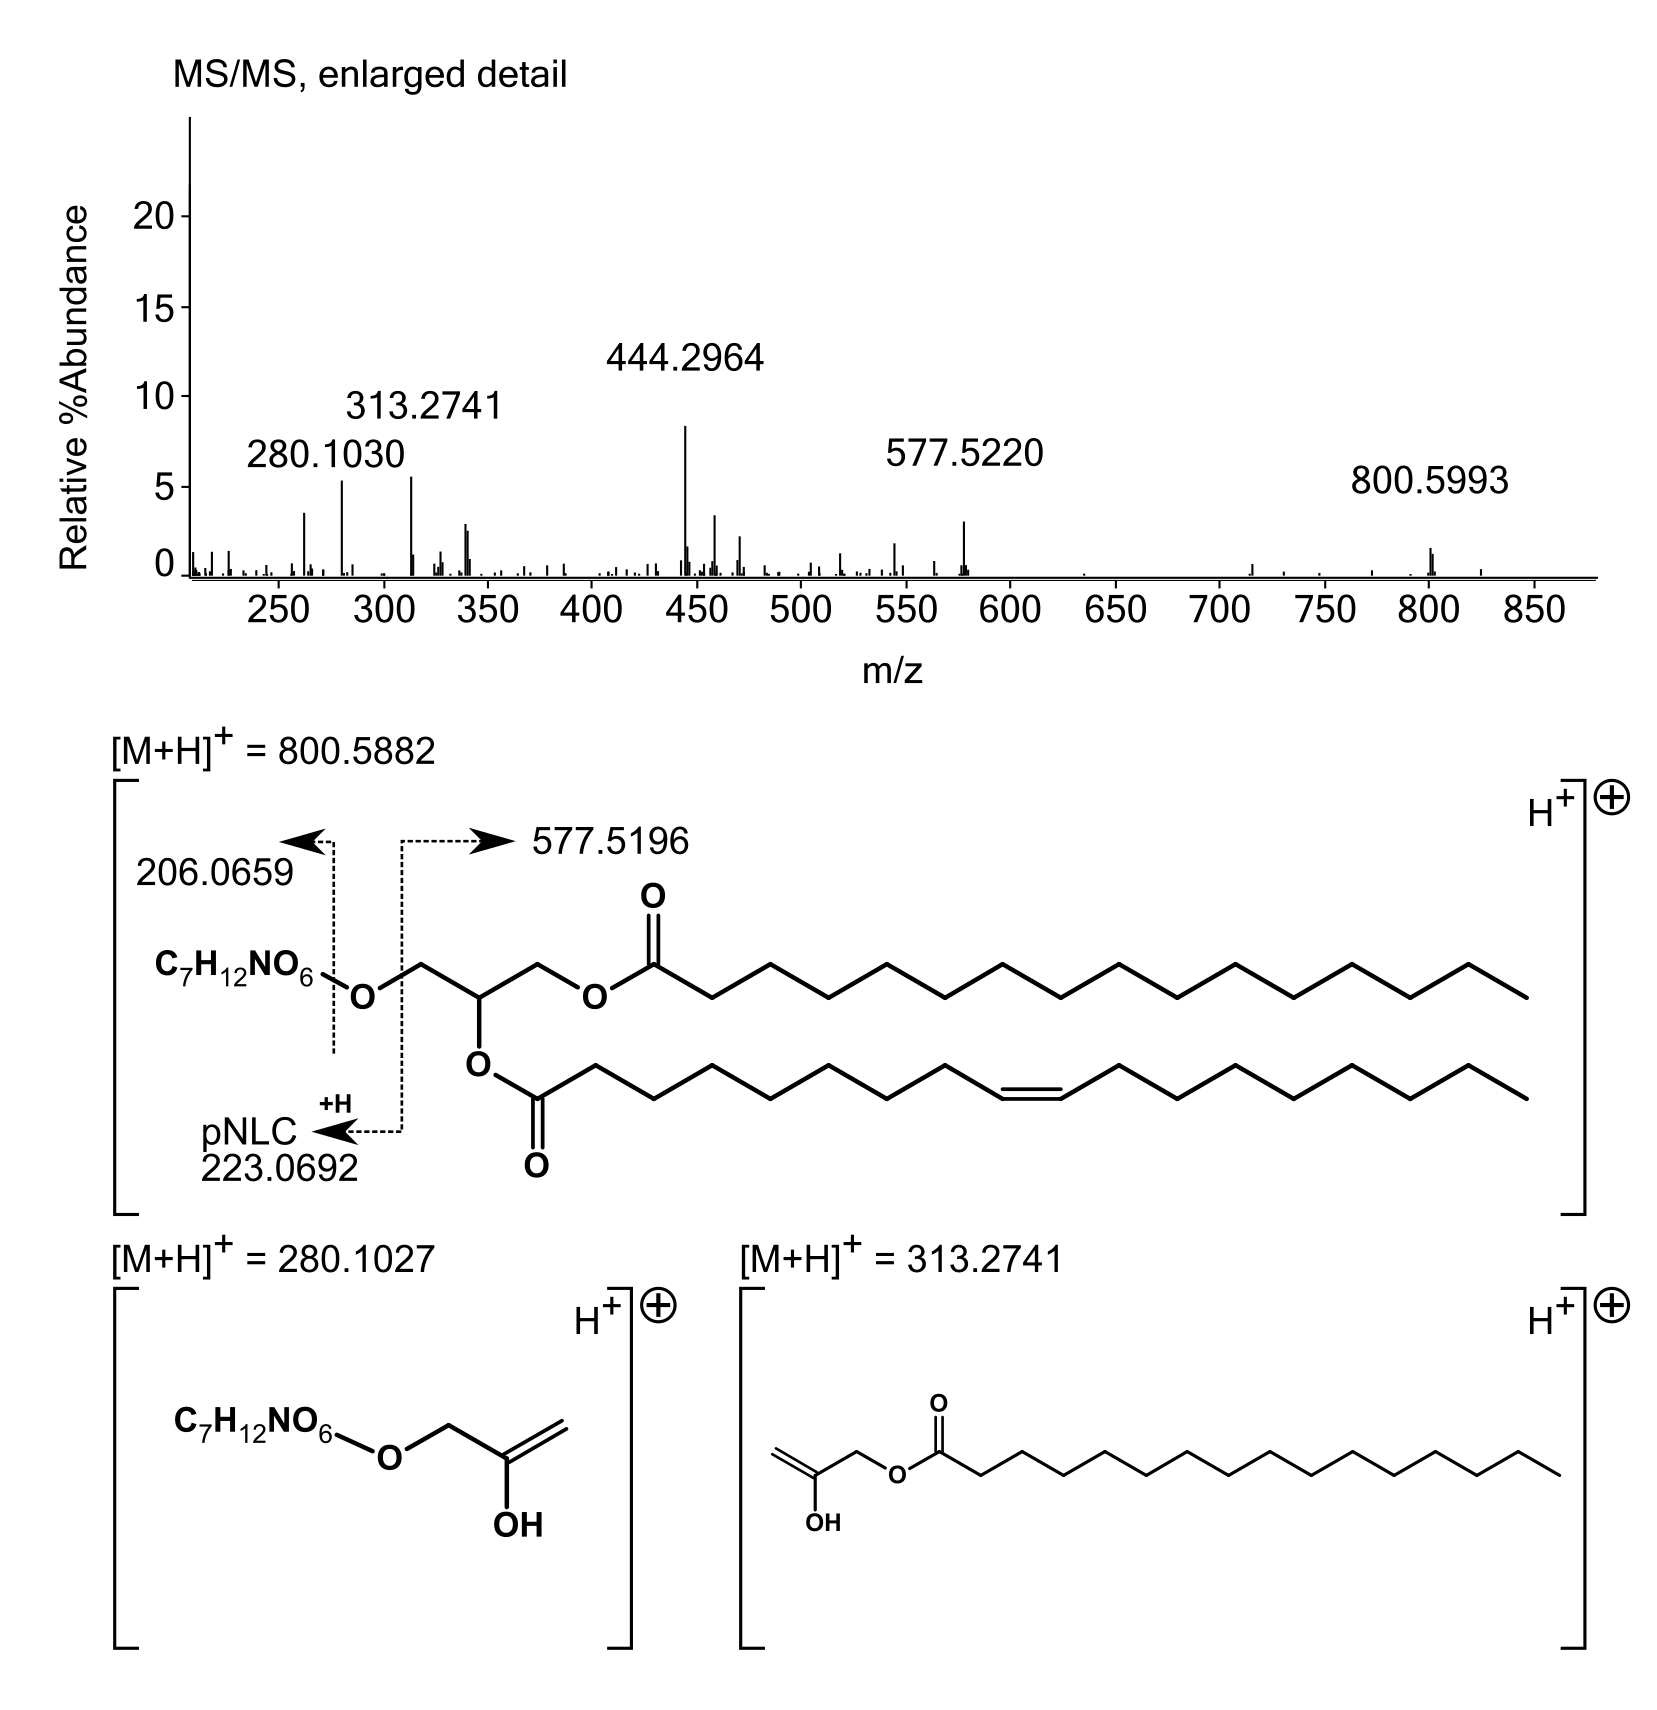
\includegraphics[width=\linewidth]{figs_app1/223-DAG_2}
       \caption{The MS/MS spectrum of C34:1 ‘223’-DAG within the m/z 140 – 250 range. The entire height of the 206 headgroup fragment is not shown. Dehydration reactions of base peak 206 results in: m/z 206.07 – 18.01 = m/z 188.06; m/z 206.07 – 2*18.01 = m/z 170.05; m/z 206.07 – 3*18.01 = m/z 152.04.}
        \label{fig:223-DAG-structure}
    \end{subfigure}
\caption{Mass spectra and putative structure for unknown lipid `223'-DAG.}
\label{fig:223-DAG}
\end{figure}
\doublespace
\clearpage
}


\afterpage{
\singlespace
\begin{figure}[h]
\centering
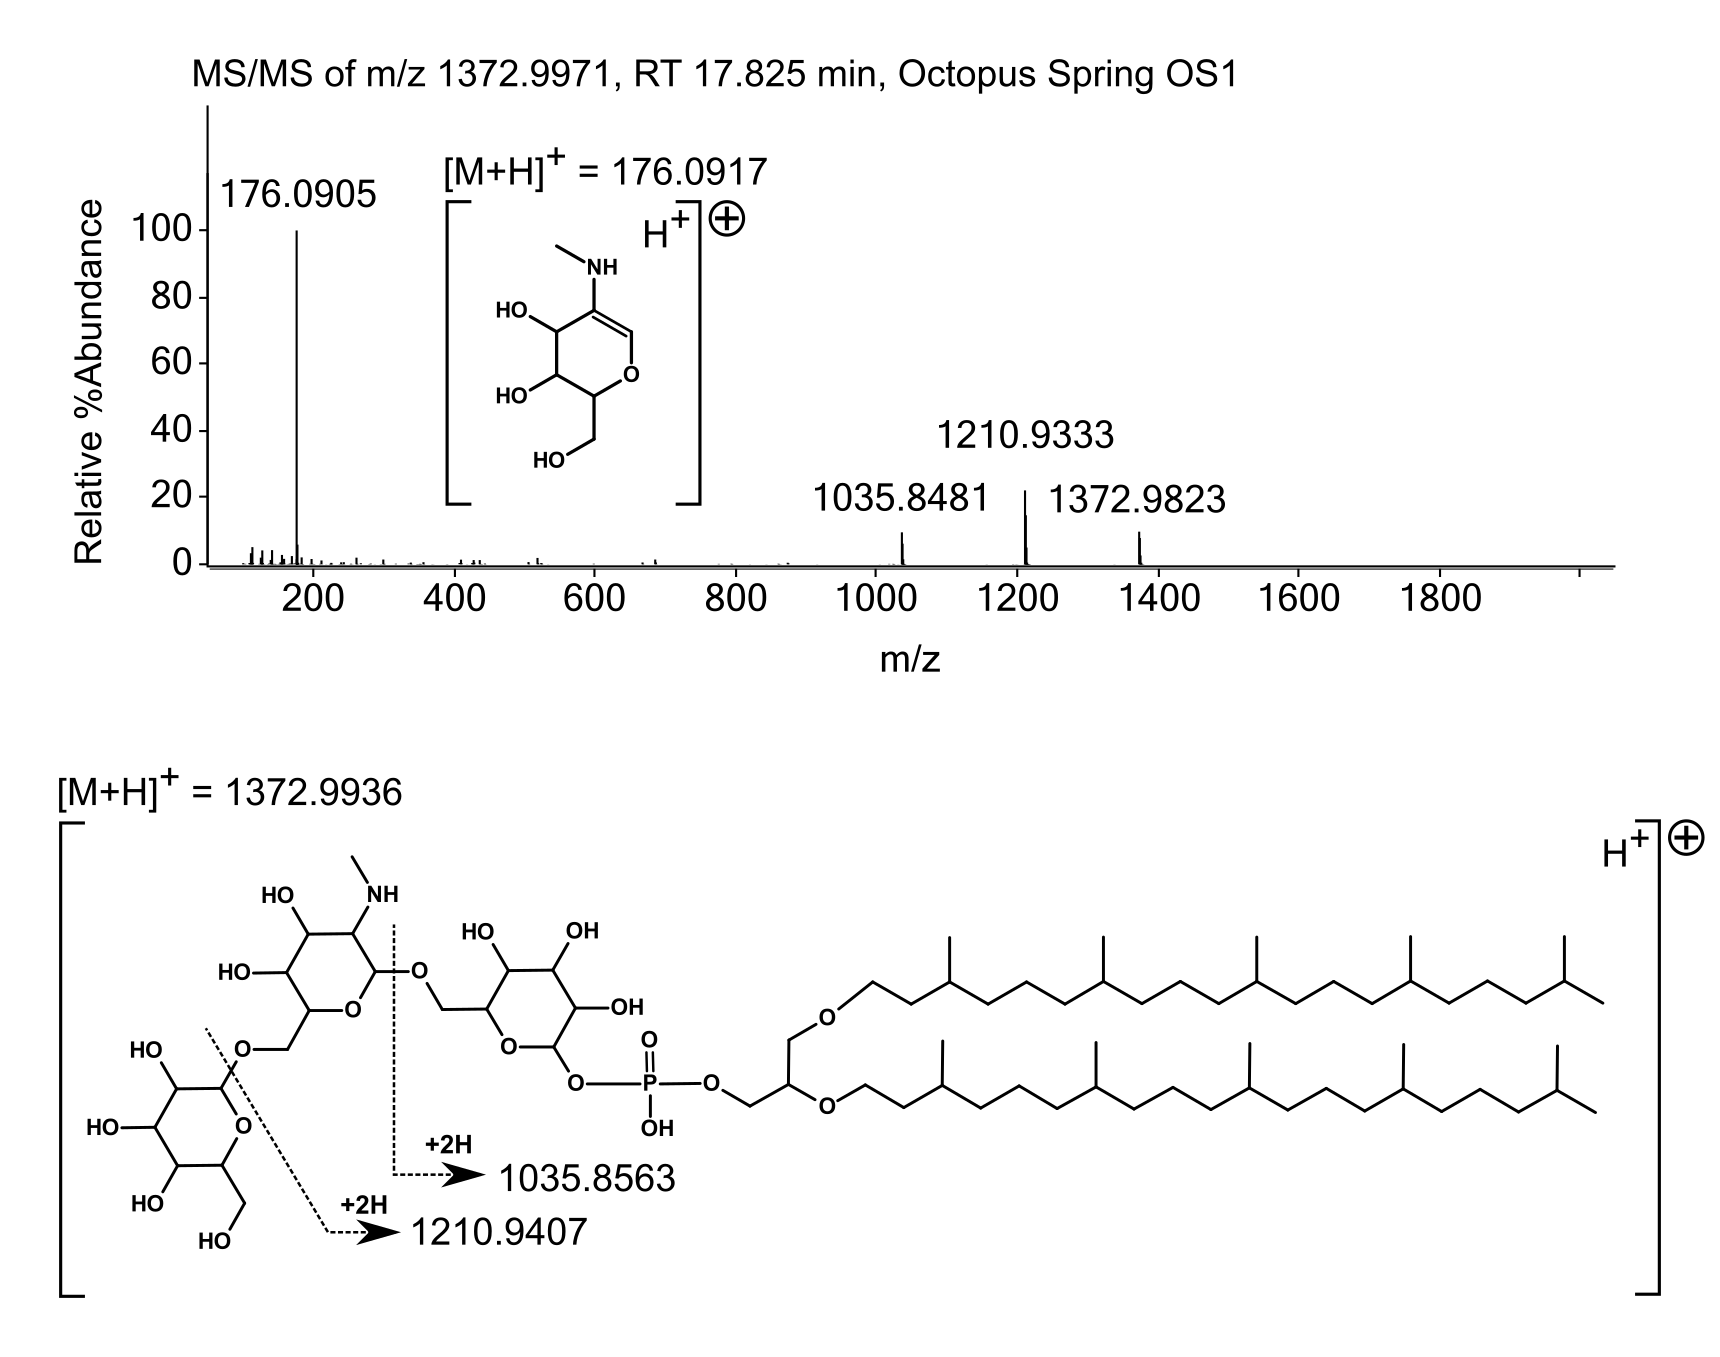
\includegraphics[width=\linewidth]{figs_app1/G-MeNG-G-P-AR}
\caption{Mass spectrum and putative structure for glycosyl (N-methyl)glycosaminyl glycosyl phosphatidylarchaeol (G-MeNG-G-P-AR).}
\label{fig:G-MeNG-G-P-AR}
\end{figure}
\doublespace
\clearpage
}

\afterpage{
\singlespace
\begin{figure}[h]
\centering
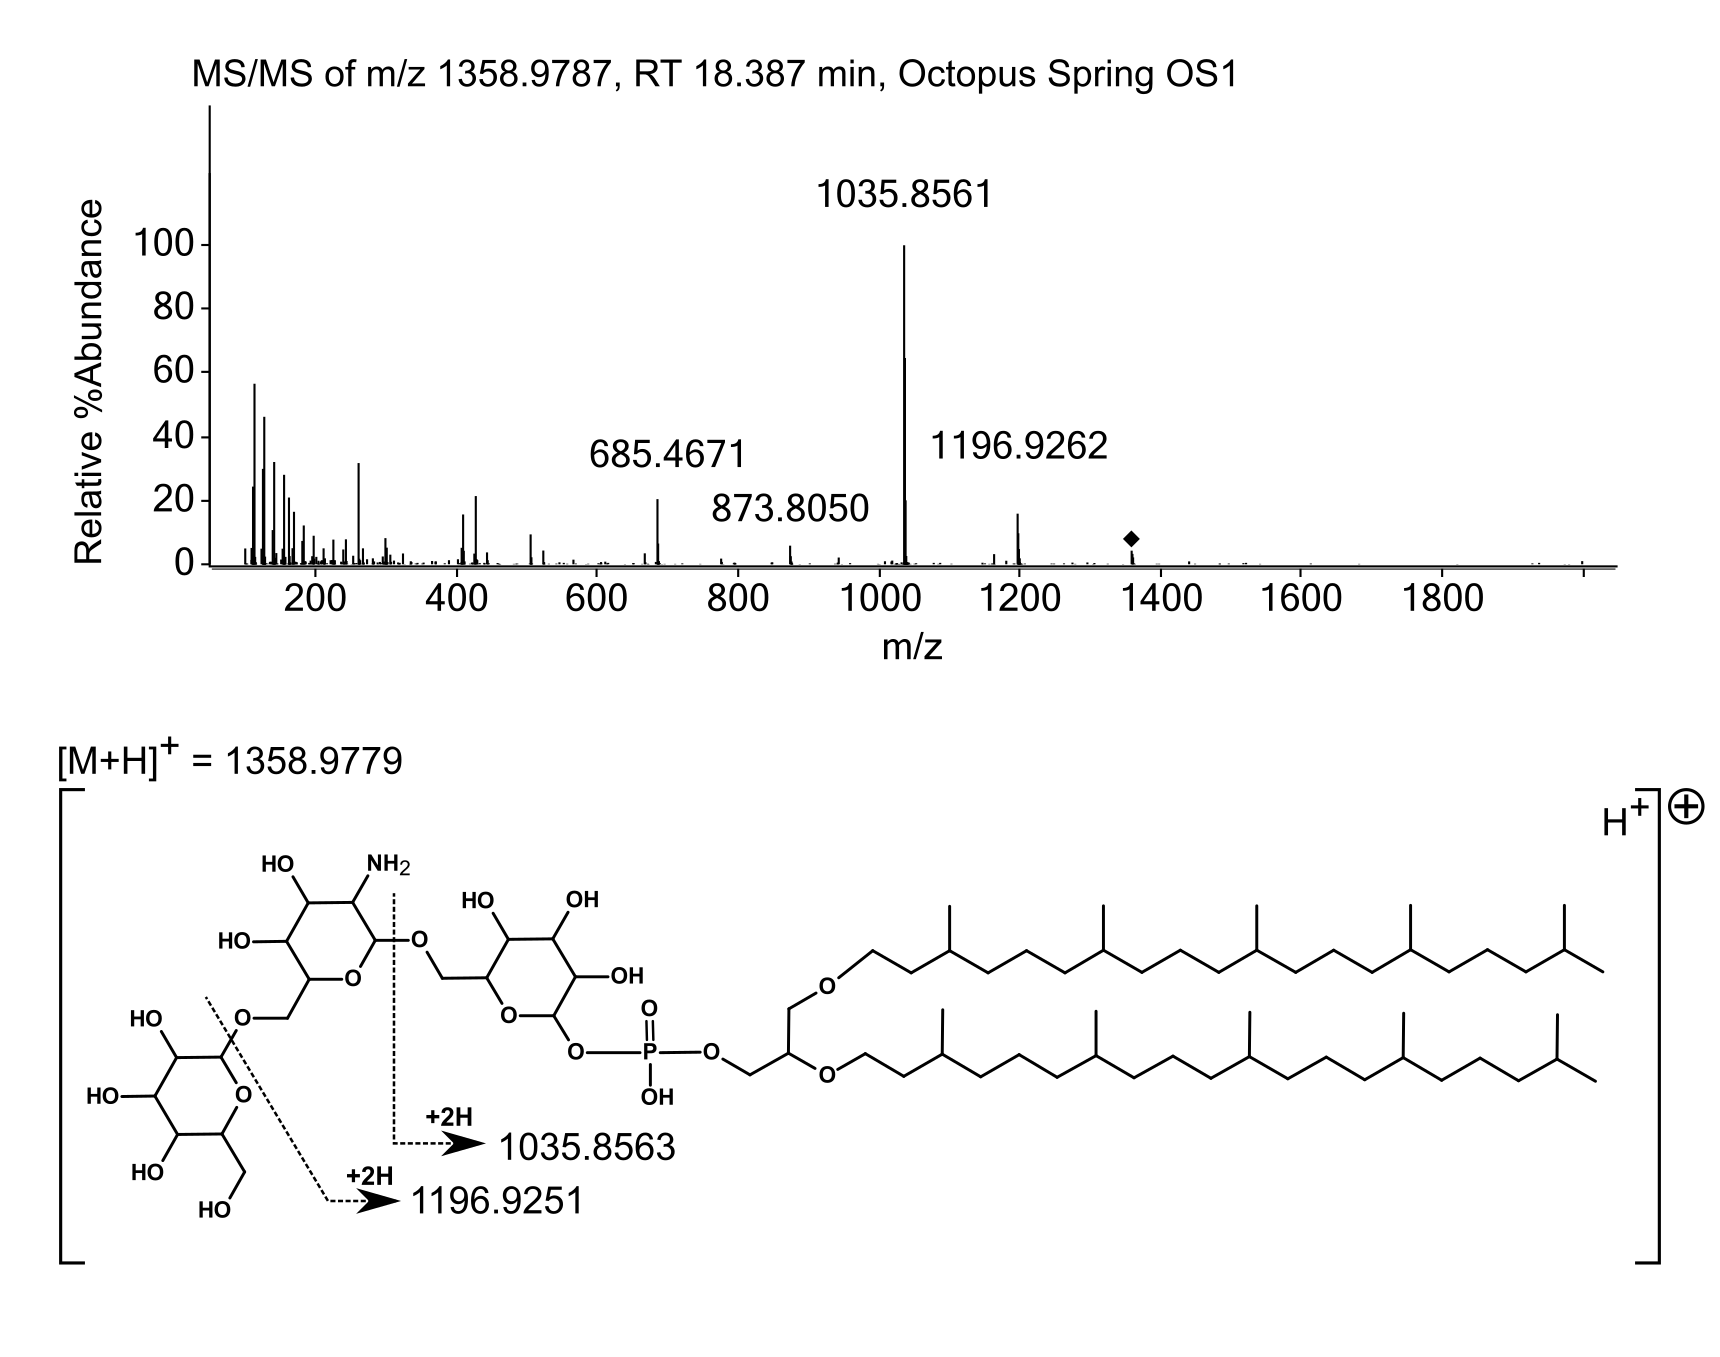
\includegraphics[width=\linewidth]{figs_app1/G-NG-G-P-AR}
\caption[Mass spectra and putative structure for glycosyl (N)glycosaminyl glycosyl phosphatidylarchaeol (G-MeNG-G-P-AR)]{Mass spectra and putative structure for glycosyl (N)glycosaminyl glycosyl phosphatidylarchaeol (G-MeNG-G-P-AR). See Figure \ref{fig:MeNG-G-P-AR} for putative structures for fragments m/z 685 and 873.}
\label{fig:G-NG-G-P-AR}
\end{figure}
\doublespace
\clearpage
}


\afterpage{
\singlespace
\begin{figure}[h]
\centering
    \begin{subfigure}[b]{1\linewidth}
       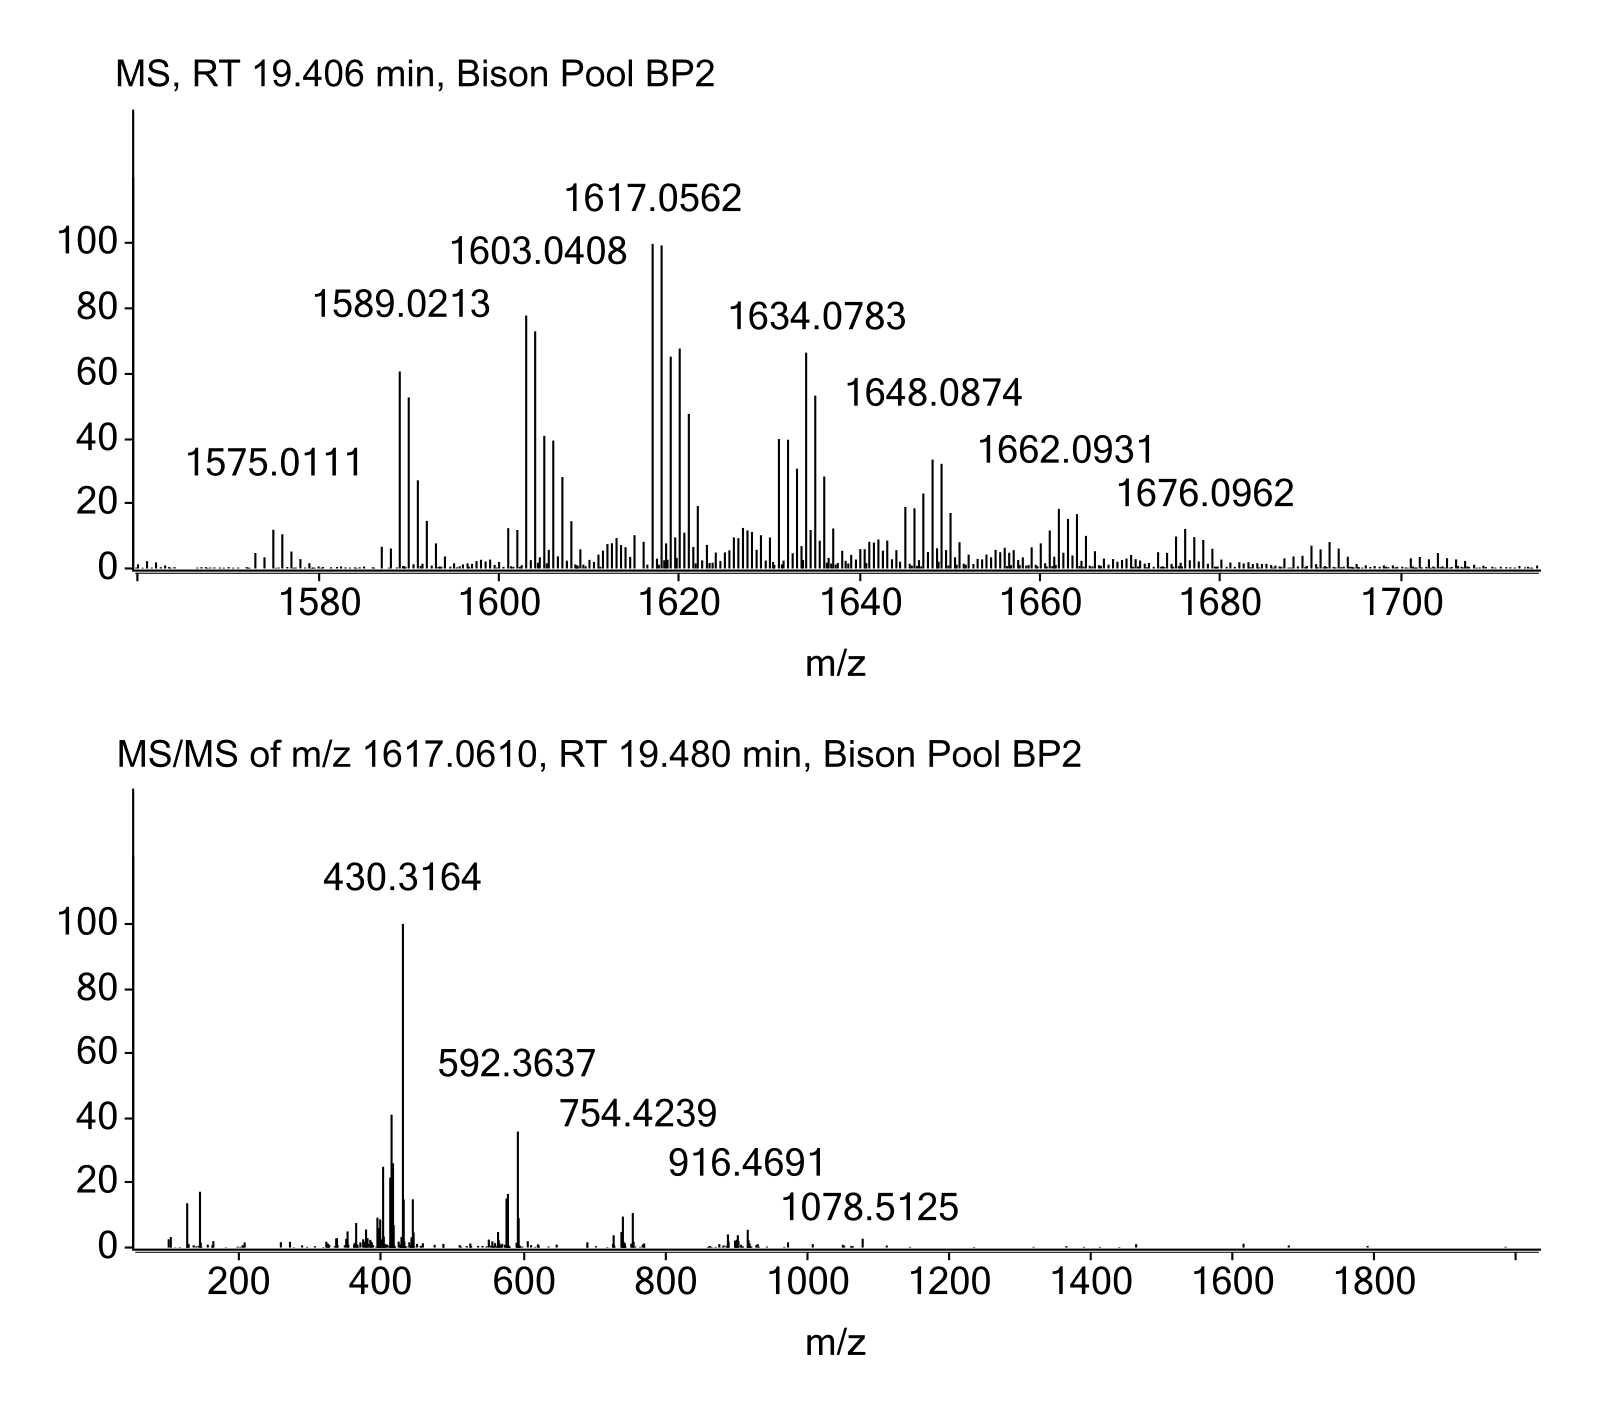
\includegraphics[width=\linewidth]{figs_app1/3G-NAcG-G_1}
       \caption{}
        \label{fig:3G-NAcG-G-MS}
    \end{subfigure}
\end{figure}
\newpage
\begin{figure}[h] \ContinuedFloat
    \begin{subfigure}[b]{1\linewidth}
       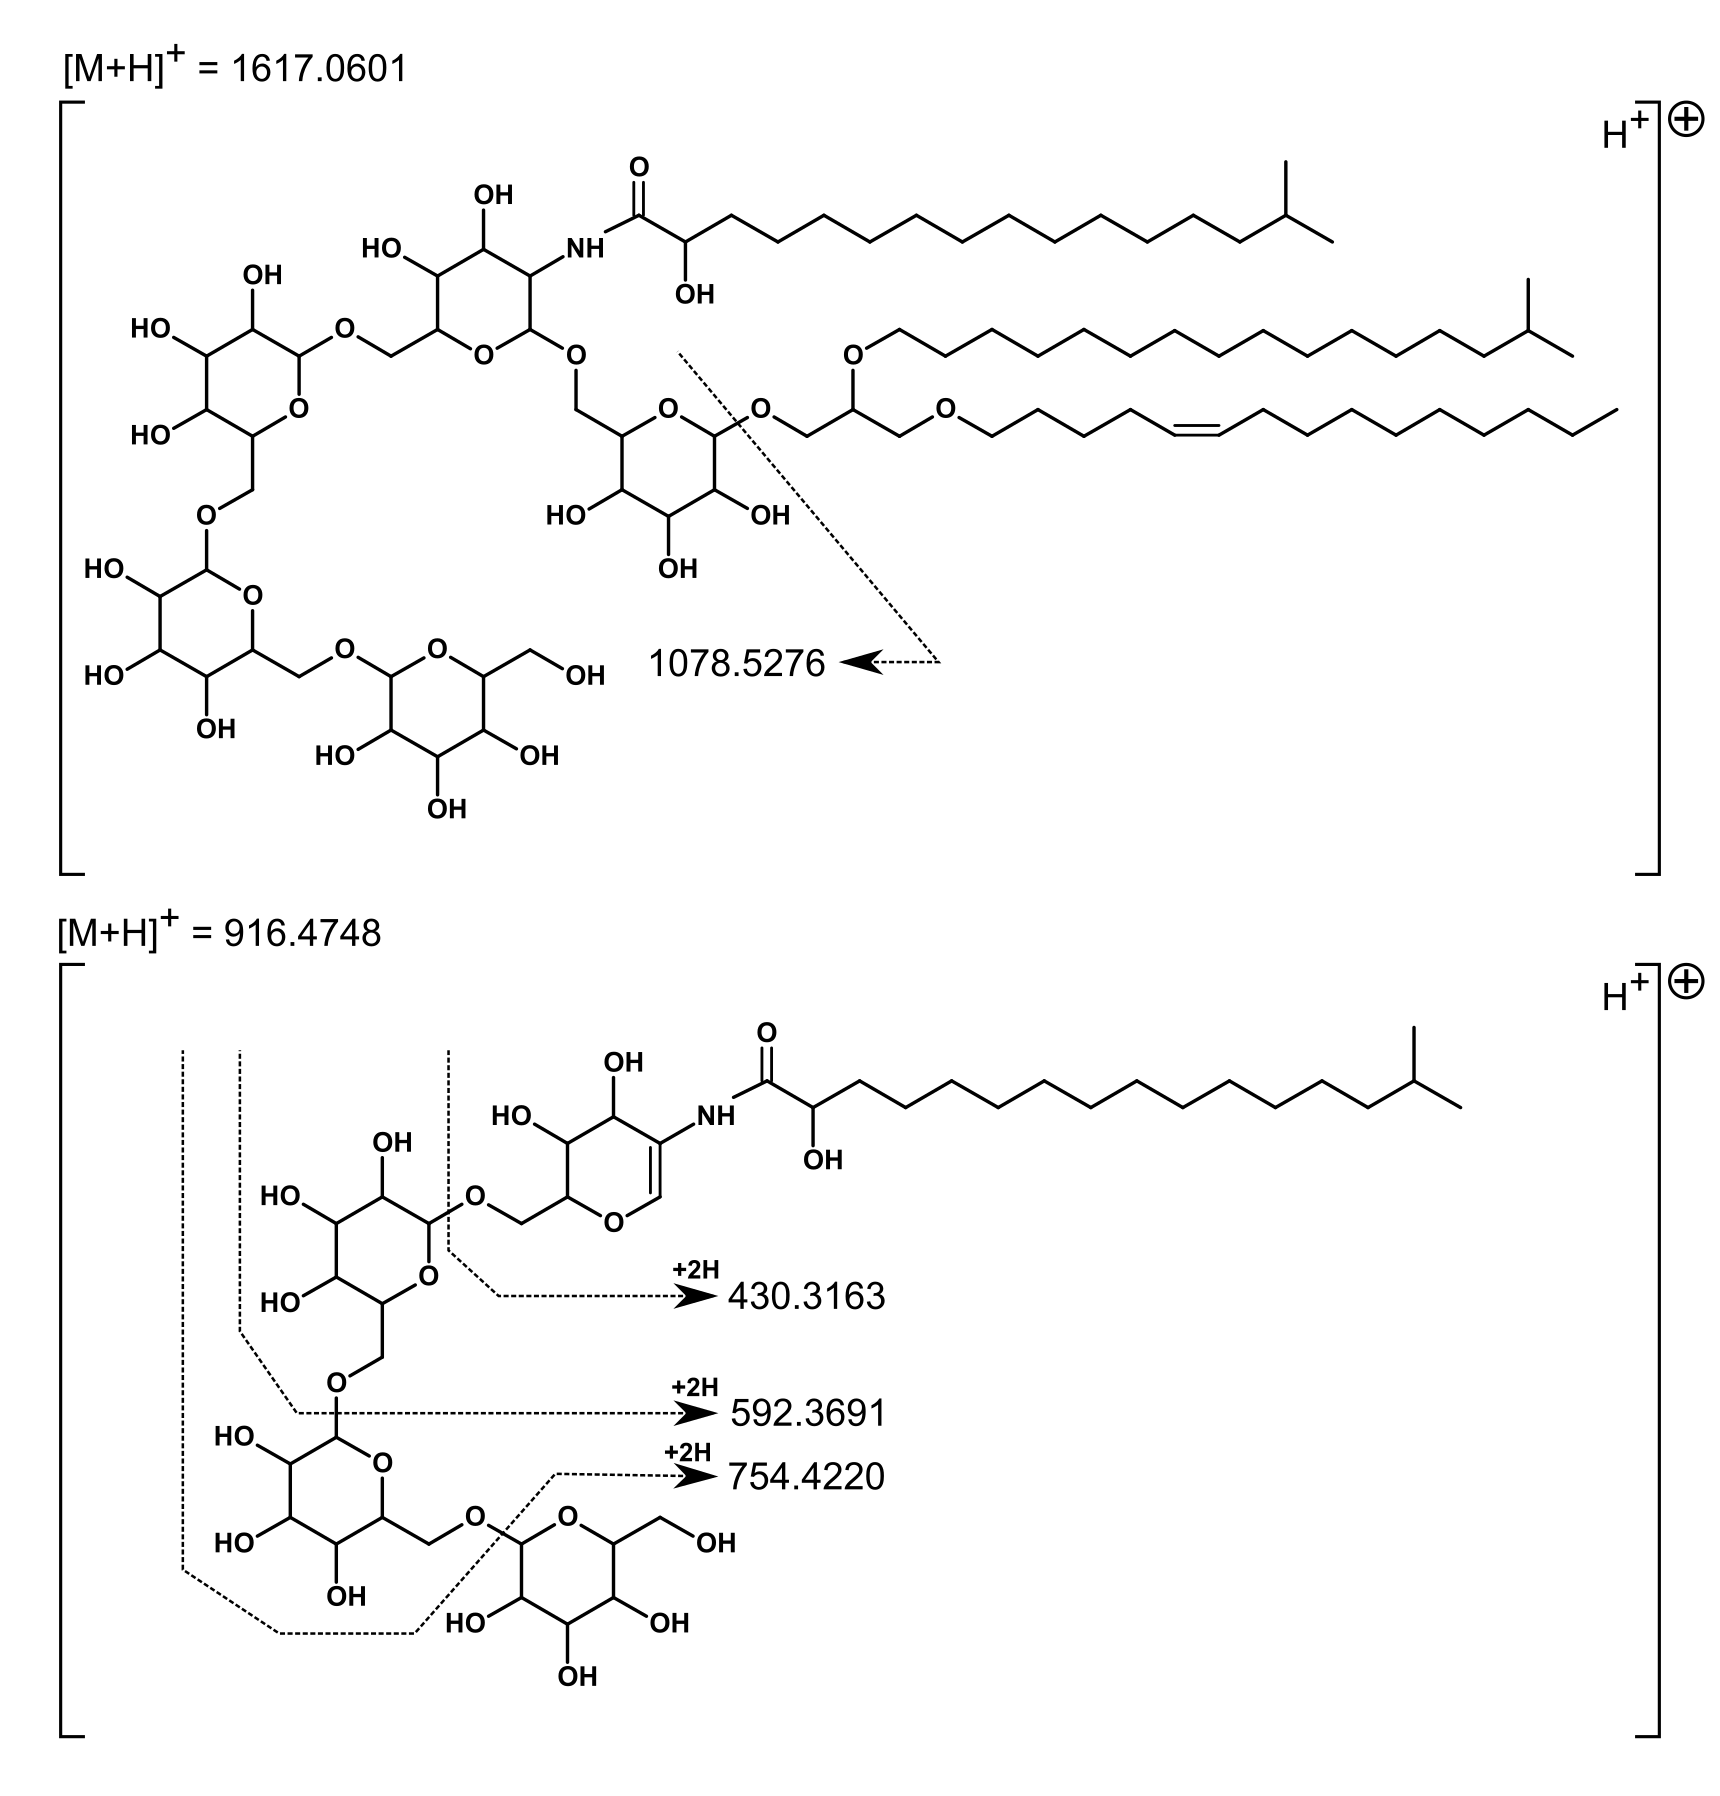
\includegraphics[width=\linewidth]{figs_app1/3G-NAcG-G_2}
       \caption{}
        \label{fig:3G-NAcG-G-structure}
    \end{subfigure}
\caption[Mass spectra and putative structure for triglycosyl (N-acetyl)glycosaminyl glycosyl dietherglycerol (3G-NAcG-G-DEG)]{(\subref{fig:3G-NAcG-G-MS}) Mass spectra and (\subref{fig:3G-NAcG-G-structure}) putative structure for triglycosyl (N-acetyl)glycosaminyl glycosyl dietherglycerol (3G-NAcG-G-DEG).}
\label{fig:3G-NAcG-G}
\end{figure}
\doublespace
\clearpage
}

\afterpage{
\singlespace
\begin{figure}[h]
       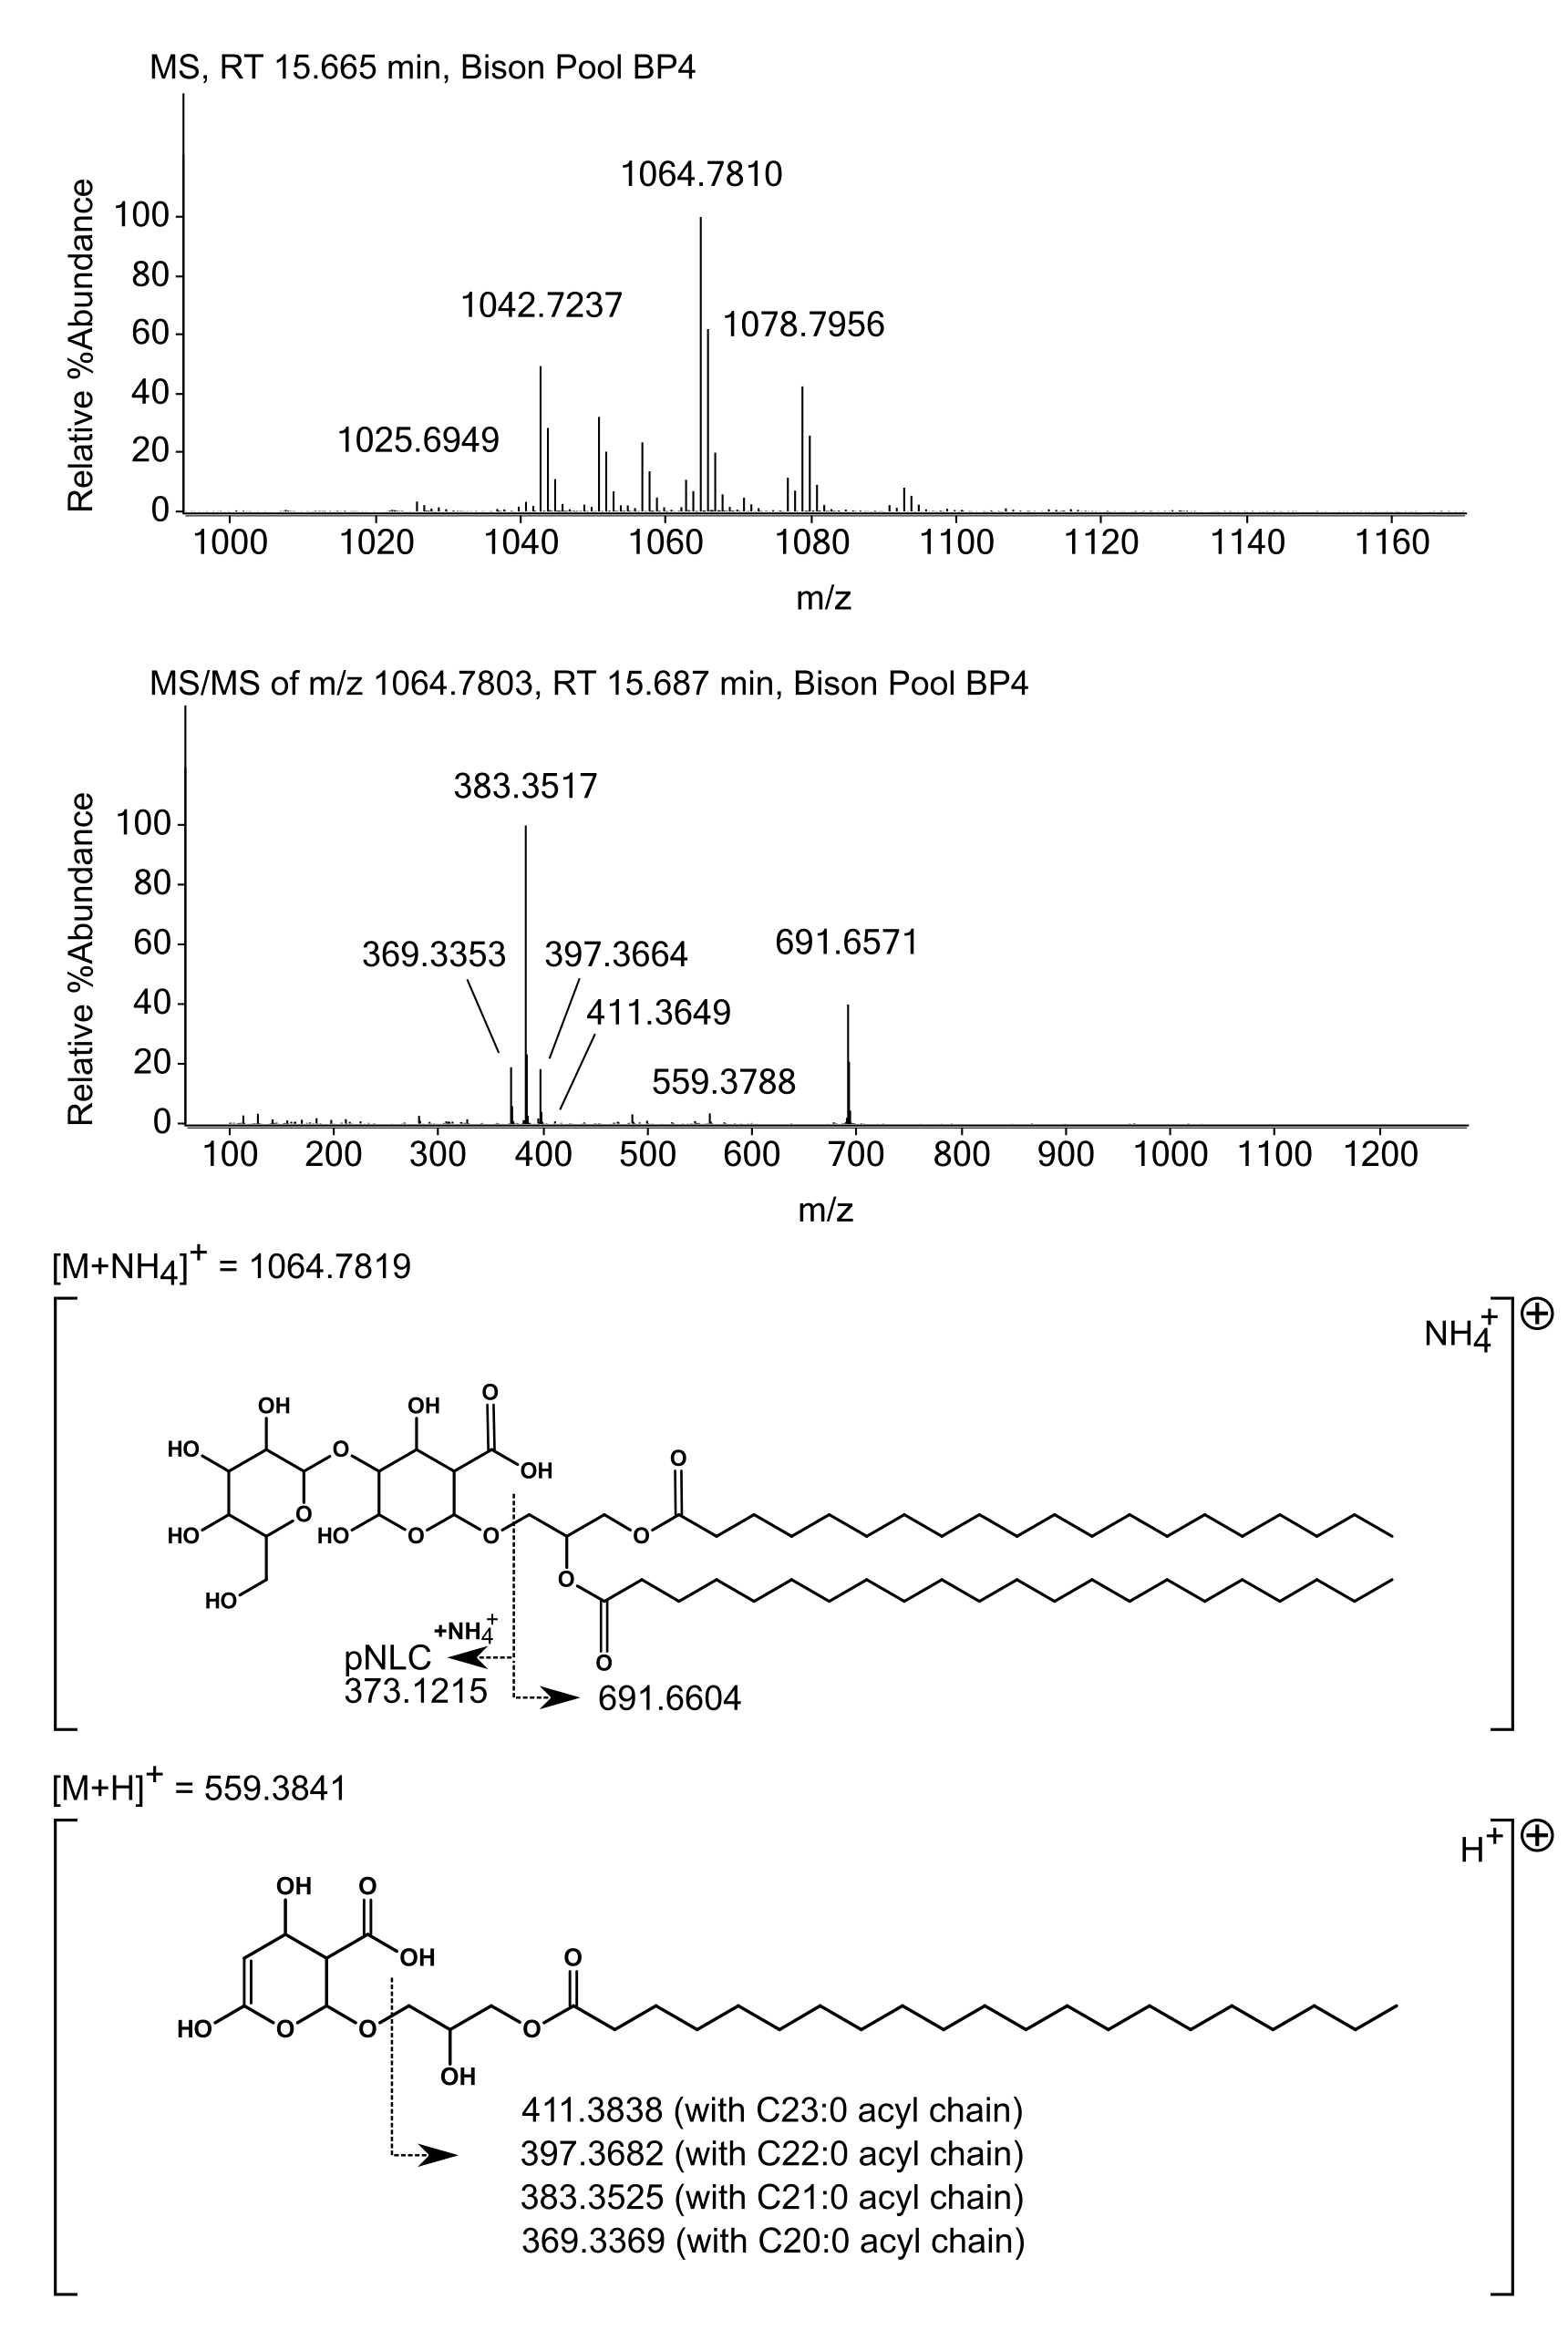
\includegraphics[width=0.9\linewidth]{figs_app1/G-GA-DAG}
       \caption{Mass spectra and putative structure for G-GA-DAG.}
\label{fig:G-GA-DAG}
\end{figure}
\doublespace
\clearpage
}